% !TEX program = tectonic
\documentclass[preprint,12pt]{elsarticle}
\biboptions{numbers}

% ─── Language & encoding ────────────────────────────────────
\usepackage{iftex}
\usepackage[T1]{fontenc}
\ifPDFTeX
  \usepackage[utf8]{inputenc}
\fi
\usepackage{lmodern}
\usepackage[english]{babel}
\usepackage{silence}
\usepackage{microtype}

% ─── Math ────────────────────────────────────────────────────
\usepackage{amsmath,amssymb,amsthm}

% ─── Tables & figures ───────────────────────────────────────
\usepackage{booktabs}
\usepackage{tabularx}
\usepackage{multirow}
\usepackage{xcolor}
\usepackage{graphicx}
\usepackage{float}
\usepackage{placeins}
\usepackage{caption}
\usepackage{subcaption}
\usepackage{tikz}
\usetikzlibrary{arrows.meta,positioning,fit,calc,shapes.geometric}
\newcolumntype{Y}{>{\raggedright\arraybackslash}X}
\newcolumntype{L}[1]{>{\raggedright\arraybackslash}p{#1}}
\setlength{\emergencystretch}{3em}
\hfuzz=20pt
\hbadness=10000
\vbadness=10000
\raggedbottom
\setlength{\textfloatsep}{7pt plus 1pt minus 2pt}
\setlength{\floatsep}{6pt plus 1pt minus 1pt}
\setlength{\intextsep}{7pt plus 1pt minus 1pt}
\setcounter{topnumber}{5}
\setcounter{bottomnumber}{4}
\setcounter{totalnumber}{8}
\renewcommand{\topfraction}{0.95}
\renewcommand{\bottomfraction}{0.85}
\renewcommand{\textfraction}{0.05}
\renewcommand{\floatpagefraction}{0.75}
\makeatletter
\setlength{\@fptop}{0pt}
\setlength{\@fpsep}{8pt plus 1fil}
\setlength{\@fpbot}{0pt plus 1fil}
\makeatother

% ─── Algorithms ──────────────────────────────────────────────
\usepackage[ruled,linesnumbered,noend]{algorithm2e}
\SetKwComment{Comment}{$\triangleright$~}{}

% ─── Hyperlinks ──────────────────────────────────────────────
\usepackage{hyperref}
\hypersetup{
  colorlinks=true,
  linkcolor=black,
  citecolor=black,
  urlcolor=blue,
}
\urlstyle{same}
\usepackage{orcidlink}
\usepackage[capitalise,noabbrev]{cleveref}

% ─── Code listings ───────────────────────────────────────────
\usepackage{listings}
\lstset{
  basicstyle=\ttfamily\small,
  breaklines=true,
  frame=single,
  columns=fullflexible,
}

% ─── Theorem environments ────────────────────────────────────
\newtheorem{theorem}{Theorem}[section]
\newtheorem{lemma}[theorem]{Lemma}
\newtheorem{corollary}[theorem]{Corollary}
\newtheorem{proposition}[theorem]{Proposition}
\newtheorem{securityclaim}[theorem]{Security claim}
\crefname{securityclaim}{security claim}{security claims}
\Crefname{securityclaim}{Security claim}{Security claims}
\theoremstyle{definition}
\newtheorem{definition}[theorem]{Definition}
\newtheorem{remark}[theorem]{Remark}

% ─── Notation macros ────────────────────────────────────────
\newcommand{\tech}[1]{\textnormal{#1}}
\newcommand{\domain}[1]{\textnormal{``#1''}}
\renewcommand{\mathsf}[1]{\mathrm{#1}}
\newcommand{\secpar}{\lambda}
\newcommand{\negl}{\mathrm{negl}}
\newcommand{\ppt}{\mathrm{PPT}}
\newcommand{\adv}{\mathbf{Adv}}
\newcommand{\advA}{\mathcal{A}}
\newcommand{\advB}{\mathcal{B}}
\newcommand{\advS}{\mathcal{S}}
\newcommand{\challenger}{\mathcal{C}}
\newcommand{\oracle}{\mathcal{O}}
\newcommand{\HKDF}{\tech{HKDF}}
\newcommand{\HMAC}{\tech{HMAC}}
\newcommand{\SHA}{\tech{SHA-256}}
\newcommand{\AEAD}{\tech{AES-256-GCM-SIV}}
\renewcommand{\DH}{\tech{X25519}}
\newcommand{\KEM}{\tech{ML-KEM-768}}
\newcommand{\KeyGen}{\tech{KeyGen}}
\newcommand{\Encaps}{\tech{Encaps}}
\newcommand{\Decaps}{\tech{Decaps}}
\newcommand{\Enc}{\tech{Enc}}
\newcommand{\Dec}{\tech{Dec}}
\newcommand{\GapCDH}{\tech{Gap-CDH}}
\newcommand{\INDCCA}{\tech{IND-CCA2}}
\newcommand{\INDCPA}{\tech{IND-CPA}}
\newcommand{\INTCTXT}{\tech{INT-CTXT}}
\newcommand{\MRAE}{\tech{MRAE}}
\newcommand{\PRF}{\tech{PRF}}
\newcommand{\SUFCMA}{\tech{SUF-CMA}}
\newcommand{\twoSourcePRF}{\tech{two-source PRF}}
\newcommand{\splitInputPRF}{\tech{split-input PRF}}
\newcommand{\ROM}{\tech{ROM}}
\newcommand{\eCK}{\tech{eCK}}
\newcommand{\AKE}{\tech{AKE}}
\newcommand{\concat}{\,\|\,}
\newcommand{\getsr}{\stackrel{\$}{\gets}}
\newcommand{\rk}{\mathit{rk}}
\newcommand{\ck}{\mathit{ck}}
\newcommand{\mk}{\mathit{mk}}
\newcommand{\mdk}{\mathit{mdk}}
\newcommand{\epoch}{\mathit{epoch}}
\newcommand{\IK}{\mathit{IK}}
\newcommand{\SPK}{\mathit{SPK}}
\newcommand{\EK}{\mathit{EK}}
\newcommand{\OPK}{\mathit{OPK}}
\newcommand{\Aura}{\textsc{Aura Protocol}}
\newcommand{\SPQR}{\tech{SPQR}}
\newcommand{\PQThree}{\tech{PQ3}}

\date{}

\makeatletter
\def\ps@pprintTitle{%
  \let\@oddhead\@empty
  \let\@evenhead\@empty
  \let\@oddfoot\@empty
  \let\@evenfoot\@empty}
\makeatother

% ═════════════════════════════════════════════════════════════
\begin{document}

\begin{frontmatter}

\title{Aura Protocol: Hybrid Post-Quantum Confidentiality for Secure Messaging via Per-Ratchet KEM Rotation}

\author{Oleksandr Melnychenko\texorpdfstring{\,\orcidlink{0000-0001-8565-7092}}{}\texorpdfstring{\corref{cor1}}{}}
\ead{melnychenko@khmnu.edu.ua}
\cortext[cor1]{Corresponding author.}

\address{Khmelnytskyi National University, Khmelnytskyi, Ukraine}

\journal{Journal of Information Security and Applications}

% ─────────────────────────────────────────────────────────────
% ABSTRACT
% ─────────────────────────────────────────────────────────────
\begin{abstract}
Long-lived end-to-end encrypted conversations remain exposed to
harvest-now-decrypt-later attacks when post-quantum protection is confined to
session establishment. Aura Protocol incorporates ML-KEM-768 into an
authenticated X25519 pre-key exchange and subsequent
directed ratchet transitions. The design retains classical Ed25519 identity
authentication, so its post-quantum claim concerns session-secret
confidentiality rather than post-quantum peer authentication. Each transition
combines fresh X25519 and ML-KEM contributions, binds the advertised KEM public
key through HKDF, and derives separate payload and metadata keys. The analysis
distinguishes local from two-endpoint compromise. After local compromise, the
first honest directed transition restores a classical contribution. Hybrid
recovery requires a later transition using peer DH and KEM material generated
after the compromise. Six reduction-style arguments rely on Gap-CDH, ML-KEM IND-CCA2, explicit
two-source and split-input PRF assumptions for HKDF, and misuse-resistant
authenticated-encryption assumptions.
Reduced Tamarin and ProVerif models cover selected secrecy and correspondence
properties. Implementation tests address parsing, persistence, and replay
behavior. On the evaluation host, the handshake takes $1.1$\,ms, a hybrid
transition takes $259\,\mu$s, and alternating 256-byte messages take
$280\,\mu$s per message. A hybrid ratchet carries 2{,}304 bytes of raw
DH/KEM material before serialization framing.
\end{abstract}
\vspace{-0.9\baselineskip}

\begin{keyword}
post-quantum cryptography \sep secure messaging \sep Double Ratchet \sep ML-KEM \sep post-compromise security \sep formal verification
\end{keyword}

\end{frontmatter}

% ═════════════════════════════════════════════════════════════
% 1. INTRODUCTION
% ═════════════════════════════════════════════════════════════
\section{Introduction}\label{sec:intro}

Modern asynchronous end-to-end encrypted messaging commonly combines
authenticated pre-key agreement with a stateful ratchet to obtain forward secrecy
and post-compromise security under elliptic-curve Diffie--Hellman assumptions.
X3DH and the Double Ratchet are the standard reference designs for that
pattern~\cite{signal-x3dh,cohn-gordon2020}. This design discipline is now used beyond ordinary interpersonal chat: mobile
endpoints, operational monitoring systems, and sensor-assisted field workflows
increasingly rely on asynchronous encrypted channels for coordination data, alerts,
and inspection-derived evidence~\cite{svystun2025dytam,svystun2024thermal,lysyi2025fire}.
In these settings, transcripts may remain valuable long after delivery, while
endpoint images and backups may persist for years.

A cryptographically relevant quantum computer (CRQC) would undermine the
classical assumption behind ECDH-based session secrecy. NIST has standardized
ML-KEM as a lattice-based key-encapsulation mechanism~\cite{fips203}, but
inserting a KEM into a stateful messaging protocol is not a syntactic
replacement for DH. A KEM introduces different directionality, state exposure,
ciphertext, and public-key-binding requirements. Aura Protocol is designed
around four resulting protocol constraints:

\paragraph{Challenge 1: Harvest-now-decrypt-later attacks}
An adversary that records ECDH-based traffic today could later recover affected
session secrets if a CRQC becomes available. Classical forward secrecy removes
old DH private values from endpoint state, but it does not protect a recorded
ECDH transcript once the elliptic-curve discrete logarithm problem becomes
tractable through Shor's algorithm~\cite{shor1997}.

\paragraph{Challenge 2: KEM integration granularity}
Adding a post-quantum KEM only to the initial handshake protects session
establishment, but it leaves later post-compromise recovery to the classical DH
ratchet. PQXDH~\cite{signal-pqxdh} is therefore a handshake baseline, whereas
sparse post-quantum ratchets such as \SPQR{}/Triple Ratchet~\cite{signal-spqr,signal-double-ratchet,mlkem-braid}
and periodic in-band rekeying designs such as Apple \PQThree{}~\cite{apple-pq3,stebila-pq3,linker-pq3}
are closer comparisons for continuing post-quantum state evolution. Aura
Protocol belongs to this second class: post-quantum material is refreshed inside
the ratchet state, not only at session creation.

\paragraph{Challenge 3: Directed KEM recovery in this construction}
Unlike DH, a KEM requires the encapsulation public key to be available before
the peer can contribute a ciphertext. Aura Protocol therefore uses a directed
KEM-public-key schedule and states the recovery boundary explicitly. After a
local endpoint compromise, the next honest directed step restores the classical
DH contribution. After full two-endpoint state compromise, the first
post-compromise directed step may still consume peer DH and KEM state exposed
by the compromise. Hybrid recovery is therefore tied to a later directed step
using peer material generated after the compromise. This distinction determines
the PCS claim in \cref{thm:pcs}.

\paragraph{Challenge 4: Metadata leakage}
Standard Double Ratchet envelopes expose ratchet public keys and message
counters in cleartext headers~\cite{signal-double-ratchet}. Payload encryption
alone does not hide ordering, message lifecycle, or application-level
correlation fields. Aura Protocol therefore adds an encrypted inner metadata
layer for message index, payload nonce, message type, and correlation
identifiers, while leaving delivery metadata, sizes, timing, and ratchet public
material visible.

\medskip
\noindent\textbf{Objective.} This paper specifies and evaluates a two-party
asynchronous messaging protocol that refreshes post-quantum key material at
ratchet transitions and distinguishes the recovery conditions following local
and two-endpoint compromise. The evaluation combines reduction-style analysis,
symbolic models, executable validation, and measurements of the implemented
state machine.

\medskip
\noindent\textbf{Contributions and novelty.} Aura Protocol contributes a
two-party construction for directed hybrid ratcheting. Sparse post-quantum ratcheting
(\SPQR{}/ML-KEM Braid~\cite{signal-spqr,signal-double-ratchet,mlkem-braid})
and periodic in-band rekeying (Apple \PQThree{}~\cite{apple-pq3,stebila-pq3,linker-pq3})
are the closest modern baselines. Against that background, the paper makes four
contributions:

\begin{enumerate}
  \item \textbf{N1: directed hybrid ratcheting and recovery.} Every direction change triggers an X25519 and ML-KEM-768 update. The resulting PCS statement separates one-step classical recovery after local compromise from delayed hybrid recovery after full two-endpoint compromise (\cref{thm:pcs}).

  \item \textbf{N2: HKDF binding of ratchet KEM keys.} Each fresh ML-KEM public key enters the HKDF info parameter during ratchet key derivation. Substitution changes the derived root state and causes the subsequent AEAD check to fail, which binds the accepted KEM key without a per-ratchet signature (\cref{lem:augmented-hkdf}).

  \item \textbf{N3: two-layer AEAD with metadata-key rotation.} Envelope metadata and payload bytes use separate keys. The metadata key rotates by ratchet epoch, and both layers use AES-256-GCM-SIV to limit the consequences of nonce reuse (\cref{lem:two-layer}).

  \item \textbf{N4: implementation-backed evaluation.} Reduction-style arguments and reduced symbolic models are paired with executable checks of parsing, ratchet atomicity, replay handling, sealed-state persistence, and the measured cost of the two-party implementation.
\end{enumerate}

\begin{table}[H]
\centering
\caption{Contribution-to-evidence map for the two-party Aura Protocol scope.}
\label{tab:contribution-map}
\footnotesize
\setlength{\tabcolsep}{2pt}
\begin{tabularx}{\textwidth}{@{}L{0.08\textwidth}L{0.28\textwidth}Y@{}}
\toprule
ID & Research claim & Main evidence in this paper \\
\midrule
N1 & Directed hybrid ratcheting can refresh DH and KEM material beyond the initial handshake. & PCS claim (\cref{thm:pcs}), ratchet algorithm (\cref{alg:send-ratchet}), ratchet benchmarks (\cref{tab:bench-core,tab:bench-overhead}). \\
N2 & HKDF-info binding makes KEM public-key substitution a state mismatch rather than a silent downgrade. & Augmented-binding lemma (\cref{lem:augmented-hkdf}), manipulation traces (\cref{tab:kem-binding-traces}), tamper/rejection validation. \\
N3 & Metadata and payload protection can be separated without merging their key domains. & Two-layer AEAD lemma (\cref{lem:two-layer}), metadata taxonomy (\cref{tab:metadata-boundary}), envelope processing tests. \\
N4 & The implemented state machine preserves the protocol's rejection, replay, persistence, and cost assumptions. & Verification-scope table (\cref{tab:verification-scope}), validation map (\cref{tab:test-proof-mapping}), operational invariants (\cref{sec:operational-invariants}), and benchmark results. \\
\bottomrule
\end{tabularx}
\end{table}

% ═════════════════════════════════════════════════════════════
% 2. RELATED WORK
% ═════════════════════════════════════════════════════════════
\section{Related Work}\label{sec:related}

\paragraph{Signal protocol}
The Signal protocol, formalized by Cohn-Gordon et al.~\cite{cohn-gordon2020}, achieves forward secrecy and post-compromise security through the combination of X3DH key agreement~\cite{signal-x3dh} and the Double Ratchet algorithm. Its ratcheting behavior has received detailed symbolic and computational analysis~\cite{cohn-gordon2020,alwen2020,bienstock2020}. Its DH-derived session keys do not protect recorded traffic against a future adversary able to solve elliptic-curve discrete logarithms.

\paragraph{Post-quantum extensions to Signal}
Signal's PQXDH protocol~\cite{signal-pqxdh} adds a post-quantum KEM encapsulation at session establishment, with Kyber-1024 used in the specification's example instantiation. Brendel et al.~\cite{brendel2020} propose a generic post-quantum X3DH construction, and Hashimoto et al.~\cite{hashimoto2021} provide an efficient instantiation. These works are natural baselines for harvest-now-decrypt-later protection at session establishment, but not for post-quantum post-compromise recovery in a long-lived channel.

Signal \SPQR{}/Triple Ratchet~\cite{signal-spqr,signal-double-ratchet} is the relevant Signal-family comparison point for ongoing post-quantum state evolution. It runs a sparse post-quantum ratchet alongside the classical Double Ratchet and combines their message keys. Its ML-KEM Braid component is specified as a Sparse Continuous Key Agreement protocol~\cite{mlkem-braid}. For a current comparison, PQXDH is therefore only the handshake baseline.

\paragraph{Industrial post-quantum messaging}
Apple \PQThree{}~\cite{apple-pq3,stebila-pq3,linker-pq3} also moves post-quantum material beyond the initial handshake through periodic in-band rekeying, and has public reduction-style and Tamarin analyses. It is a deployed baseline with a closed implementation. Aura Protocol occupies a complementary position: it gives an open two-party construction whose distinctive mechanisms are ratchet-level KEM-key binding, metadata-key rotation, and a separately stated validation boundary.

\paragraph{Ratcheting analysis}
Alwen et al.~\cite{alwen2020} and Bienstock et al.~\cite{bienstock2020} give detailed analyses of Double Ratchet security notions, modularization, and post-compromise recovery. This line of work motivates the separation between the state-evolution claim and the concrete implementation invariants studied here.

\paragraph{Hybrid key exchange}
The concept of hybrid key exchange---combining classical and post-quantum primitives---has been studied for Internet key exchange and TLS, including early CECPQ2 deployment experiments~\cite{cecpq2}, Open Quantum Safe work~\cite{stebila2020}, hybrid KEM/AKE analyses~\cite{bindel2019}, and formal TLS~1.3 analyses~\cite{dowling2020}. These works establish security under the assumption that at least one component remains secure. The combiner in \cref{thm:hybrid-combiner} follows the same principle, using HKDF with the classical shared secret as salt and the KEM shared secret as input keying material.

\paragraph{Formal verification of messaging protocols}
Tamarin~\cite{meier2013} and ProVerif~\cite{blanchet2016} have been used to verify properties of the Signal protocol~\cite{cohn-gordon2020}. The models in this paper adapt that line of analysis to a hybrid post-quantum setting, including custom equations for ML-KEM-768 and the Tamarin source-saturation issues caused by multiple DH operations.

\paragraph{Metadata privacy and anonymous delivery}
Sealed Sender~\cite{sealed-sender} hides sender identity from Signal's service, while mix-network designs such as Sphinx~\cite{sphinx} and Loopix~\cite{loopix} address network-level anonymity. Aura Protocol's metadata layer is narrower: it encrypts protocol envelope fields under rotating per-ratchet-epoch keys, complementing rather than replacing sender-hiding delivery systems.

\paragraph{Nonce-misuse-resistant AEAD}
AES-256-GCM-SIV~\cite{rfc8452} provides misuse-resistant authenticated encryption, degrading to deterministic authenticated encryption under nonce reuse, whereas AES-GCM loses its standard confidentiality and integrity bounds under repeated nonces. Rogaway and Shrimpton~\cite{rogaway2006} formalize the MRAE security notion. Aura Protocol uses GCM-SIV to provide residual authenticity and deterministic leakage bounds alongside monotonic nonce counters.


% ═════════════════════════════════════════════════════════════
% 3. PRELIMINARIES
% ═════════════════════════════════════════════════════════════
\section{Preliminaries}\label{sec:prelim}

\subsection{Notation}

Let $\secpar$ denote the security parameter. A function $f(\secpar)$ is \emph{negligible} if $f(\secpar) \in o(\secpar^{-c})$ for every constant $c > 0$. We write this as $f \in \negl(\secpar)$. All algorithms are implicitly parameterized by $\secpar$. The notation $x \getsr S$ denotes uniform random sampling from a finite set $S$. The operator $\concat$ denotes byte-string concatenation, and $\ppt$ denotes probabilistic polynomial-time.

An \emph{epoch} in this paper means a ratchet epoch: the interval of session
state governed by one root key, one active sending or receiving chain key, and
one metadata key. The epoch counter increments when a directed hybrid ratchet
step installs fresh DH and ML-KEM material. Multiple same-direction messages may
belong to the same epoch. They are distinguished by the per-chain message
index $n$.

\begin{table}[tbp]
\centering
\caption{Protocol-specific notation.}\label{tab:notation}
\small
\begin{tabularx}{\textwidth}{@{}L{2.4cm}X@{}}
\toprule
Symbol & Meaning \\
\midrule
$\IK_X$ & Long-term X25519 identity keypair of party $X$ \\
$\SPK_X$ & Signed pre-key (X25519) of party $X$ \\
$\EK_X$ & Ephemeral X25519 keypair of party $X$ \\
$\OPK_X$ & One-time pre-key (X25519) of party $X$ \\
$(kpk_X, ksk_X)$ & ML-KEM-768 keypair of party $X$ \\
$e$ & Ratchet epoch counter \\
$\rk_e$ & Root key at epoch $e$ \\
$\ck_e$ & Chain key at epoch $e$ \\
$\mk_{e,n}$ & Message key at epoch $e$, chain index $n$ \\
$\mdk_e$ & Metadata key at epoch $e$ \\
$R(\cdot)$ & Hybrid ratchet step function \\
$q_s$ & Number of sessions \\
$q_m$ & Total encrypted message attempts across all sessions \\
$N_{\max}$ & Negotiated per-chain message limit \\
\bottomrule
\end{tabularx}
\end{table}

\subsection{Cryptographic Primitives}

\begin{definition}[Diffie--Hellman on X25519]\label{def:dh}
The proof uses an idealized prime-order X25519 abstraction with
\[
  q = 2^{252} + 27742317777372353535851937790883648493 .
\]
Curve25519 has cofactor 8. The construction follows RFC~7748 clamping and rejects malformed
field encodings, small-order inputs, and all-zero shared secrets where
applicable. Cofactor and twist subtleties are not modeled beyond this
abstraction. The X25519 function~\cite{rfc7748} computes scalar multiplication
$\DH(a, B) = [a]B$ with base point $u = 9$.
\end{definition}

\begin{definition}[Gap-CDH]\label{def:gap-cdh}
The $\GapCDH$ assumption states that for all $\ppt$ adversaries $\advA$ with access to a DDH oracle $\oracle_{\mathrm{DDH}}$:
\begin{align}
  \adv^{\GapCDH}_{\DH}(\advA)
  &=
  \Pr\!\left[
    \advA^{\oracle_{\mathrm{DDH}}}(G,[a]G,[b]G) = [ab]G
  \right] \notag\\
  &\leq \negl(\secpar),
  \qquad a,b \getsr \mathbb{Z}_q .
  \label{eq:gap-cdh}
\end{align}
\end{definition}

\begin{definition}[Key Encapsulation Mechanism]\label{def:kem}
A key encapsulation mechanism $\Pi$ is specified by three algorithms with the following interfaces:
\[
  \begin{aligned}
    \KeyGen() &\to (pk, sk),\\
    \Encaps(pk) &\to (ct, ss),\\
    \Decaps(sk, ct) &\to ss.
  \end{aligned}
\]
Correctness requires
\[
  \begin{aligned}
    (ct, ss) &\gets \Encaps(pk),\\
    \Decaps(sk, ct) &= ss.
  \end{aligned}
\]
\end{definition}

\begin{definition}[IND-CCA2 for KEM]\label{def:ind-cca2}
For a key encapsulation mechanism $\Pi$, the $\INDCCA$ advantage of an adversary $\advA$ is defined as
\begin{equation}\label{eq:kem-ind-cca}
  \adv^{\INDCCA}_\Pi(\advA) = \left|\Pr\!\left[\advA^{\oracle_{\Decaps}}(pk, ct^*, ss_b) = b\right] - \frac{1}{2}\right| \leq \negl(\secpar),
\end{equation}
where $b \getsr \{0,1\}$, $(ct^*, ss_0) \gets \Encaps(pk)$, $ss_1 \getsr \{0,1\}^{256}$, and $\advA$ may not query $\oracle_{\Decaps}$ on $ct^*$.
\end{definition}

\begin{definition}[Two-Source HKDF Assumption]\label{def:dual-prf}
For the argument order used in this construction, define
\[
  F(s,k,\mathit{info}) = \HKDF(k,32,s,\mathit{info}),
\]
where $s$ is passed as the RFC~5869 salt and $k$ as input keying
material. We assume that $F$ has the $\twoSourcePRF$ property: its output is
computationally indistinguishable from random when either $s$ or $k$ is uniform
and independent, even if the other source is known or selected without access
to the fresh secret. RFC~5869 defines the extract-and-expand
interface~\cite{rfc5869}, and the HKDF analysis supplies its constructional
background~\cite{krawczyk2010}. Neither reference is cited here as a theorem for
this exact two-source combiner. The property is an explicit assumption of the
security arguments below.
\end{definition}

\begin{definition}[Split-Input Ratchet-KDF Assumption]\label{def:split-prf}
For the ratchet argument order, define
\[
  G_L(s,x,y,\mathit{info}) =
  \HKDF(x\concat y,L,s,\mathit{info}),
\]
where $s$ is the previous root key, $x$ is the X25519 contribution, and $y$
is the ML-KEM contribution. We assume that $G_L$ has the
$\splitInputPRF$ property: its output is computationally indistinguishable
from random when either $x$ or $y$ is uniform and independent, even if $s$
and the other contribution are known or selected without access to the fresh
secret. This component-robust property is not implied by the
$\twoSourcePRF$ property in \cref{def:dual-prf}: neither the salt nor the
complete concatenated input need be uniform in the ratchet game. It is an explicit assumption
of the ratchet PCS arguments rather than a theorem attributed to RFC~5869.
\end{definition}

\begin{definition}[MRAE Security~\cite{rfc8452,rogaway2006}]\label{def:mrae}
$\AEAD$ satisfies $\MRAE$ security if:
\begin{itemize}
  \item Under unique nonces: full $\INDCPA$ + $\INTCTXT$ (standard AEAD security).
  \item Under nonce reuse: degrades to deterministic authenticated encryption (DAE), leaking equality patterns for repeated $(\mathit{nonce}, \mathit{AAD}, \mathit{plaintext})$ tuples while authenticity remains governed by the $\MRAE$ bound.
\end{itemize}
\end{definition}


% ═════════════════════════════════════════════════════════════
% 4. PROTOCOL DESIGN
% ═════════════════════════════════════════════════════════════
\section{Protocol Design}\label{sec:protocol}

Aura Protocol consists of two phases: a \emph{hybrid pre-key handshake} (\cref{sec:handshake}) that establishes initial shared state, and a \emph{hybrid Double Ratchet} (\cref{sec:ratchet}) that continuously refreshes key material. Messages are protected by a \emph{two-layer AEAD} construction (\cref{sec:two-layer}). \Cref{fig:architecture} summarizes the protocol phases and the key material refreshed in each phase.

\begin{figure}[t]
\centering
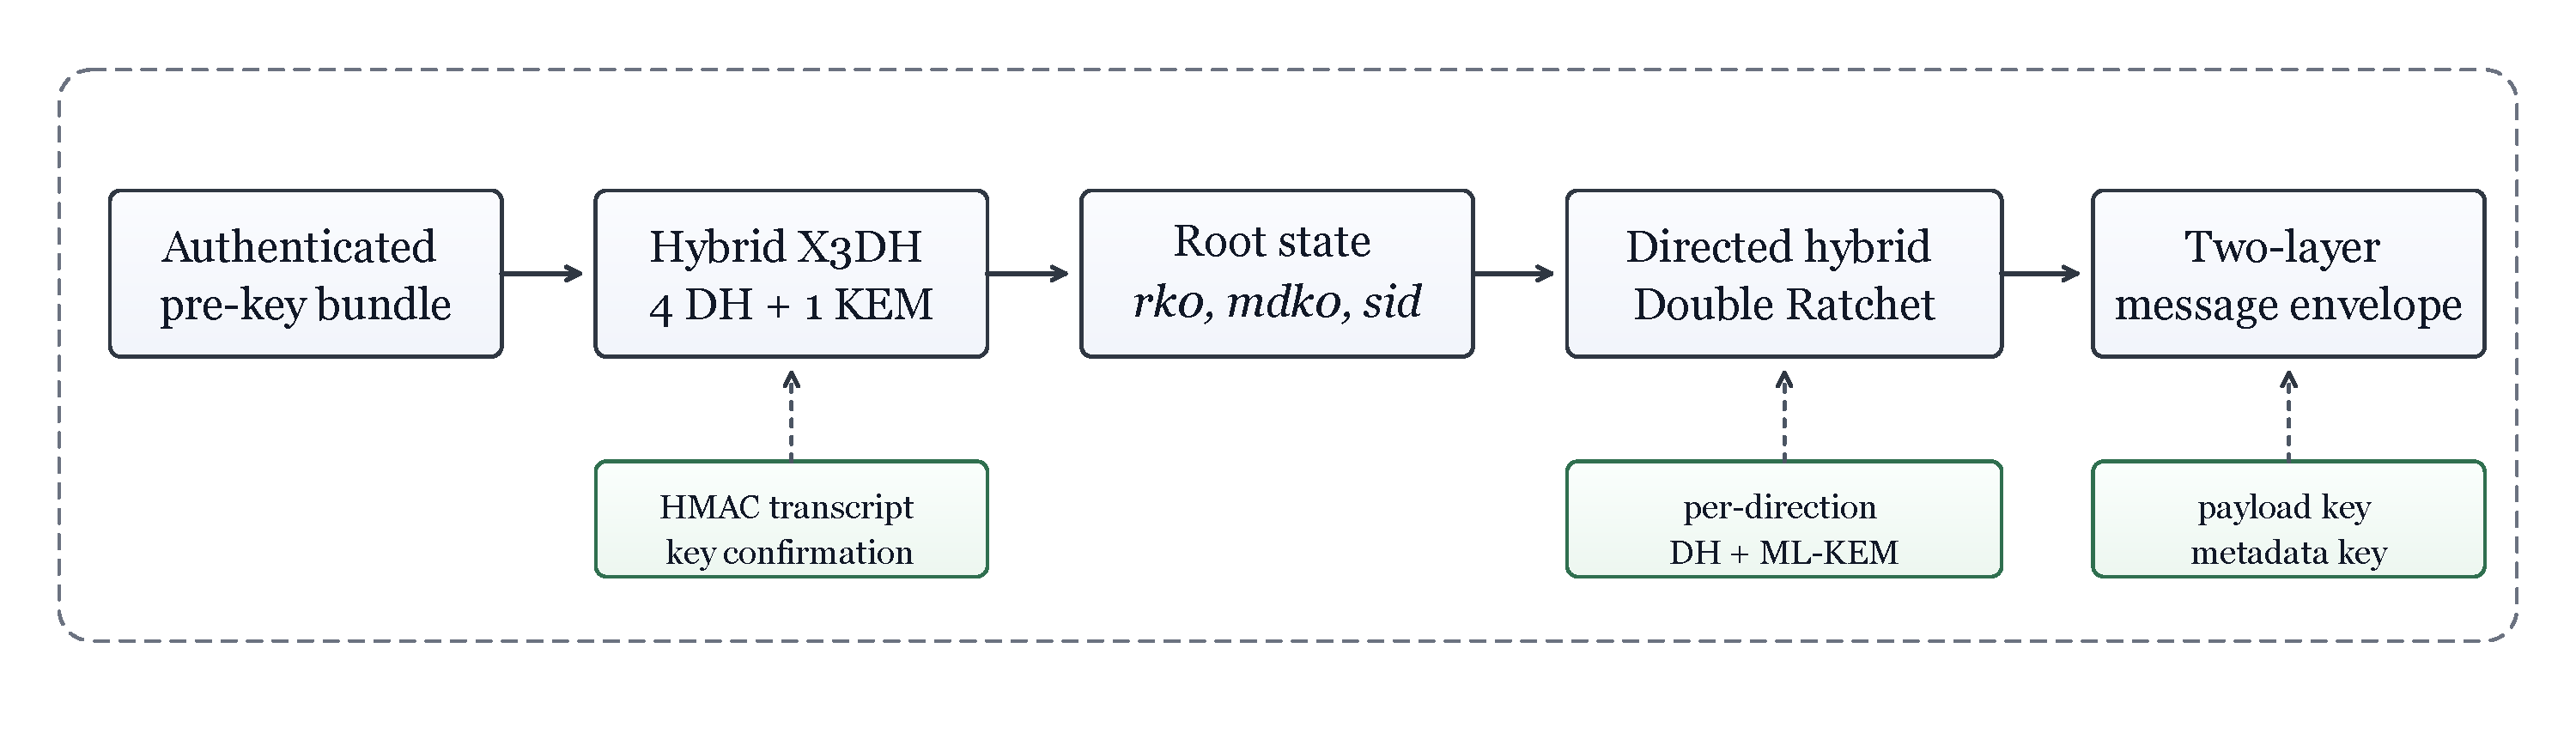
\includegraphics[width=0.98\textwidth]{figures/hybrid_x3dh_flowchart_white.pdf}
\vspace{-0.35\baselineskip}
\caption{Protocol phases and cryptographic inputs used by Aura Protocol.}\label{fig:architecture}
\end{figure}

\subsection{Pre-Key Bundle}\label{sec:bundle}

Each party $R$ publishes a pre-key bundle:
\begin{equation}\label{eq:prekey-bundle}
  \begin{aligned}
  \mathit{Bundle}_R = \bigl(&v,\; ed_R^{\mathit{pub}},\;
  \IK_R^{\mathit{pub}},\; \mathit{spk\_id},\;
  \SPK_R^{\mathit{pub}},\; \sigma_{\SPK},\\
  &\{(\mathit{opk\_id}_j,\OPK_{R,j}^{\mathit{pub}})\}_j,\;
  kpk_R,\; \sigma_{\mathit{IKX}}\bigr).
  \end{aligned}
\end{equation}
where $\sigma_{\mathit{IKX}}=\tech{Ed25519.Sign}(ed_R^{\mathit{sk}},\IK_R^{\mathit{pub}})$ binds the X25519 identity key to the Ed25519 identity key, $\sigma_{\SPK}=\tech{Ed25519.Sign}(ed_R^{\mathit{sk}},\SPK_R^{\mathit{pub}})$ signs the medium-term pre-key, $\{\OPK_{R,j}\}$ is a set of one-time pre-keys, and $kpk_R$ is the ML-KEM public key. The KEM public key is validated and transcript-bound by key confirmation. It is not treated as a separately Ed25519-signed object in this construction.

\begin{figure}[H]
\centering
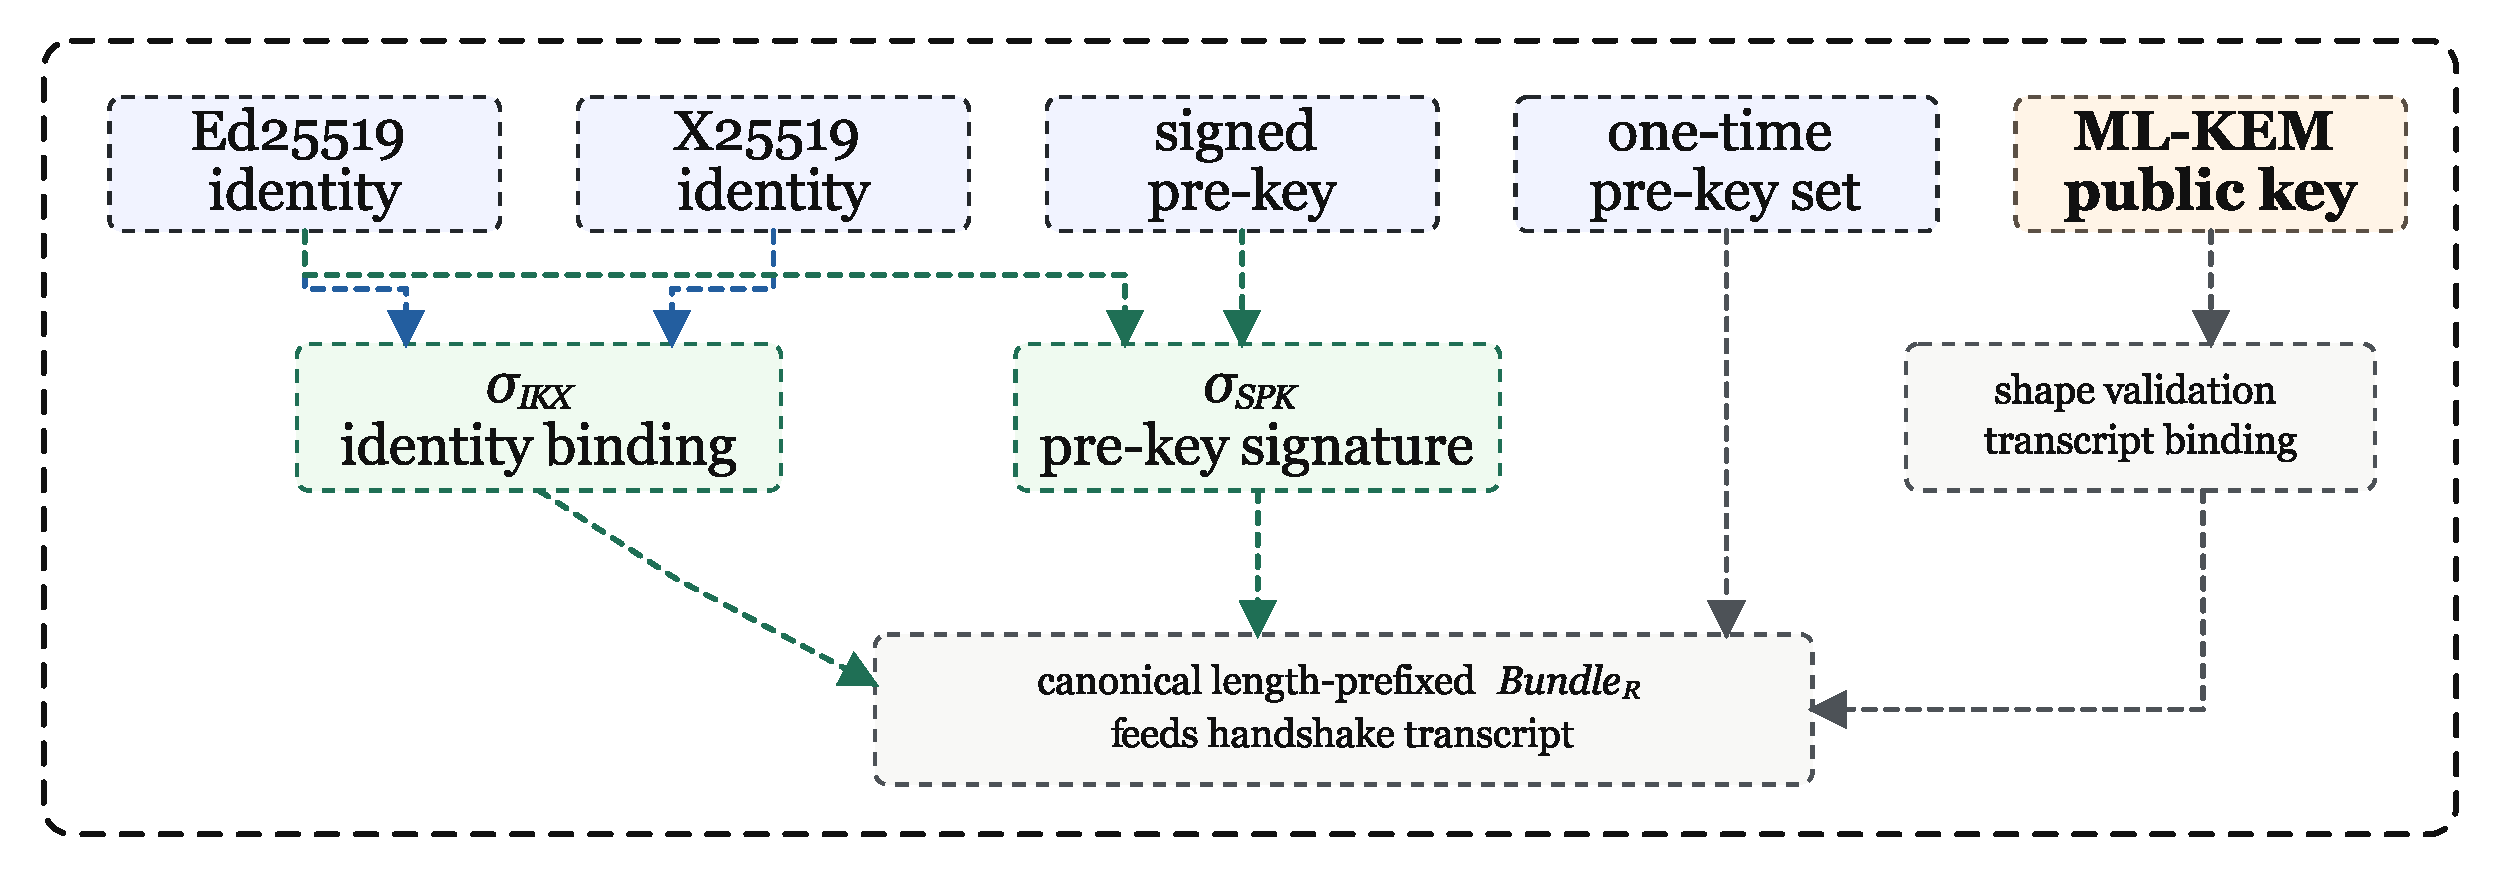
\includegraphics[width=0.98\textwidth]{figures/prekey_bundle_validation_flow_straight_arrow.pdf}
\vspace{-0.25\baselineskip}
\caption{Pre-key bundle anatomy. Classical identity and signed-pre-key fields are directly signed, while the ML-KEM public key is validated as protocol input and bound by the handshake transcript and key-confirmation MAC.}\label{fig:prekey-bundle}
\end{figure}

\subsection{Hybrid Pre-Key Agreement}\label{sec:handshake}

The initial key agreement follows the authenticated asynchronous pre-key pattern used by X3DH~\cite{signal-x3dh} and combines four X25519 Diffie--Hellman contributions with an ML-KEM-768 encapsulation and bilateral key confirmation. The message flow and root-key inputs are shown in \cref{fig:handshake-flow}.

\begin{figure}[H]
\centering
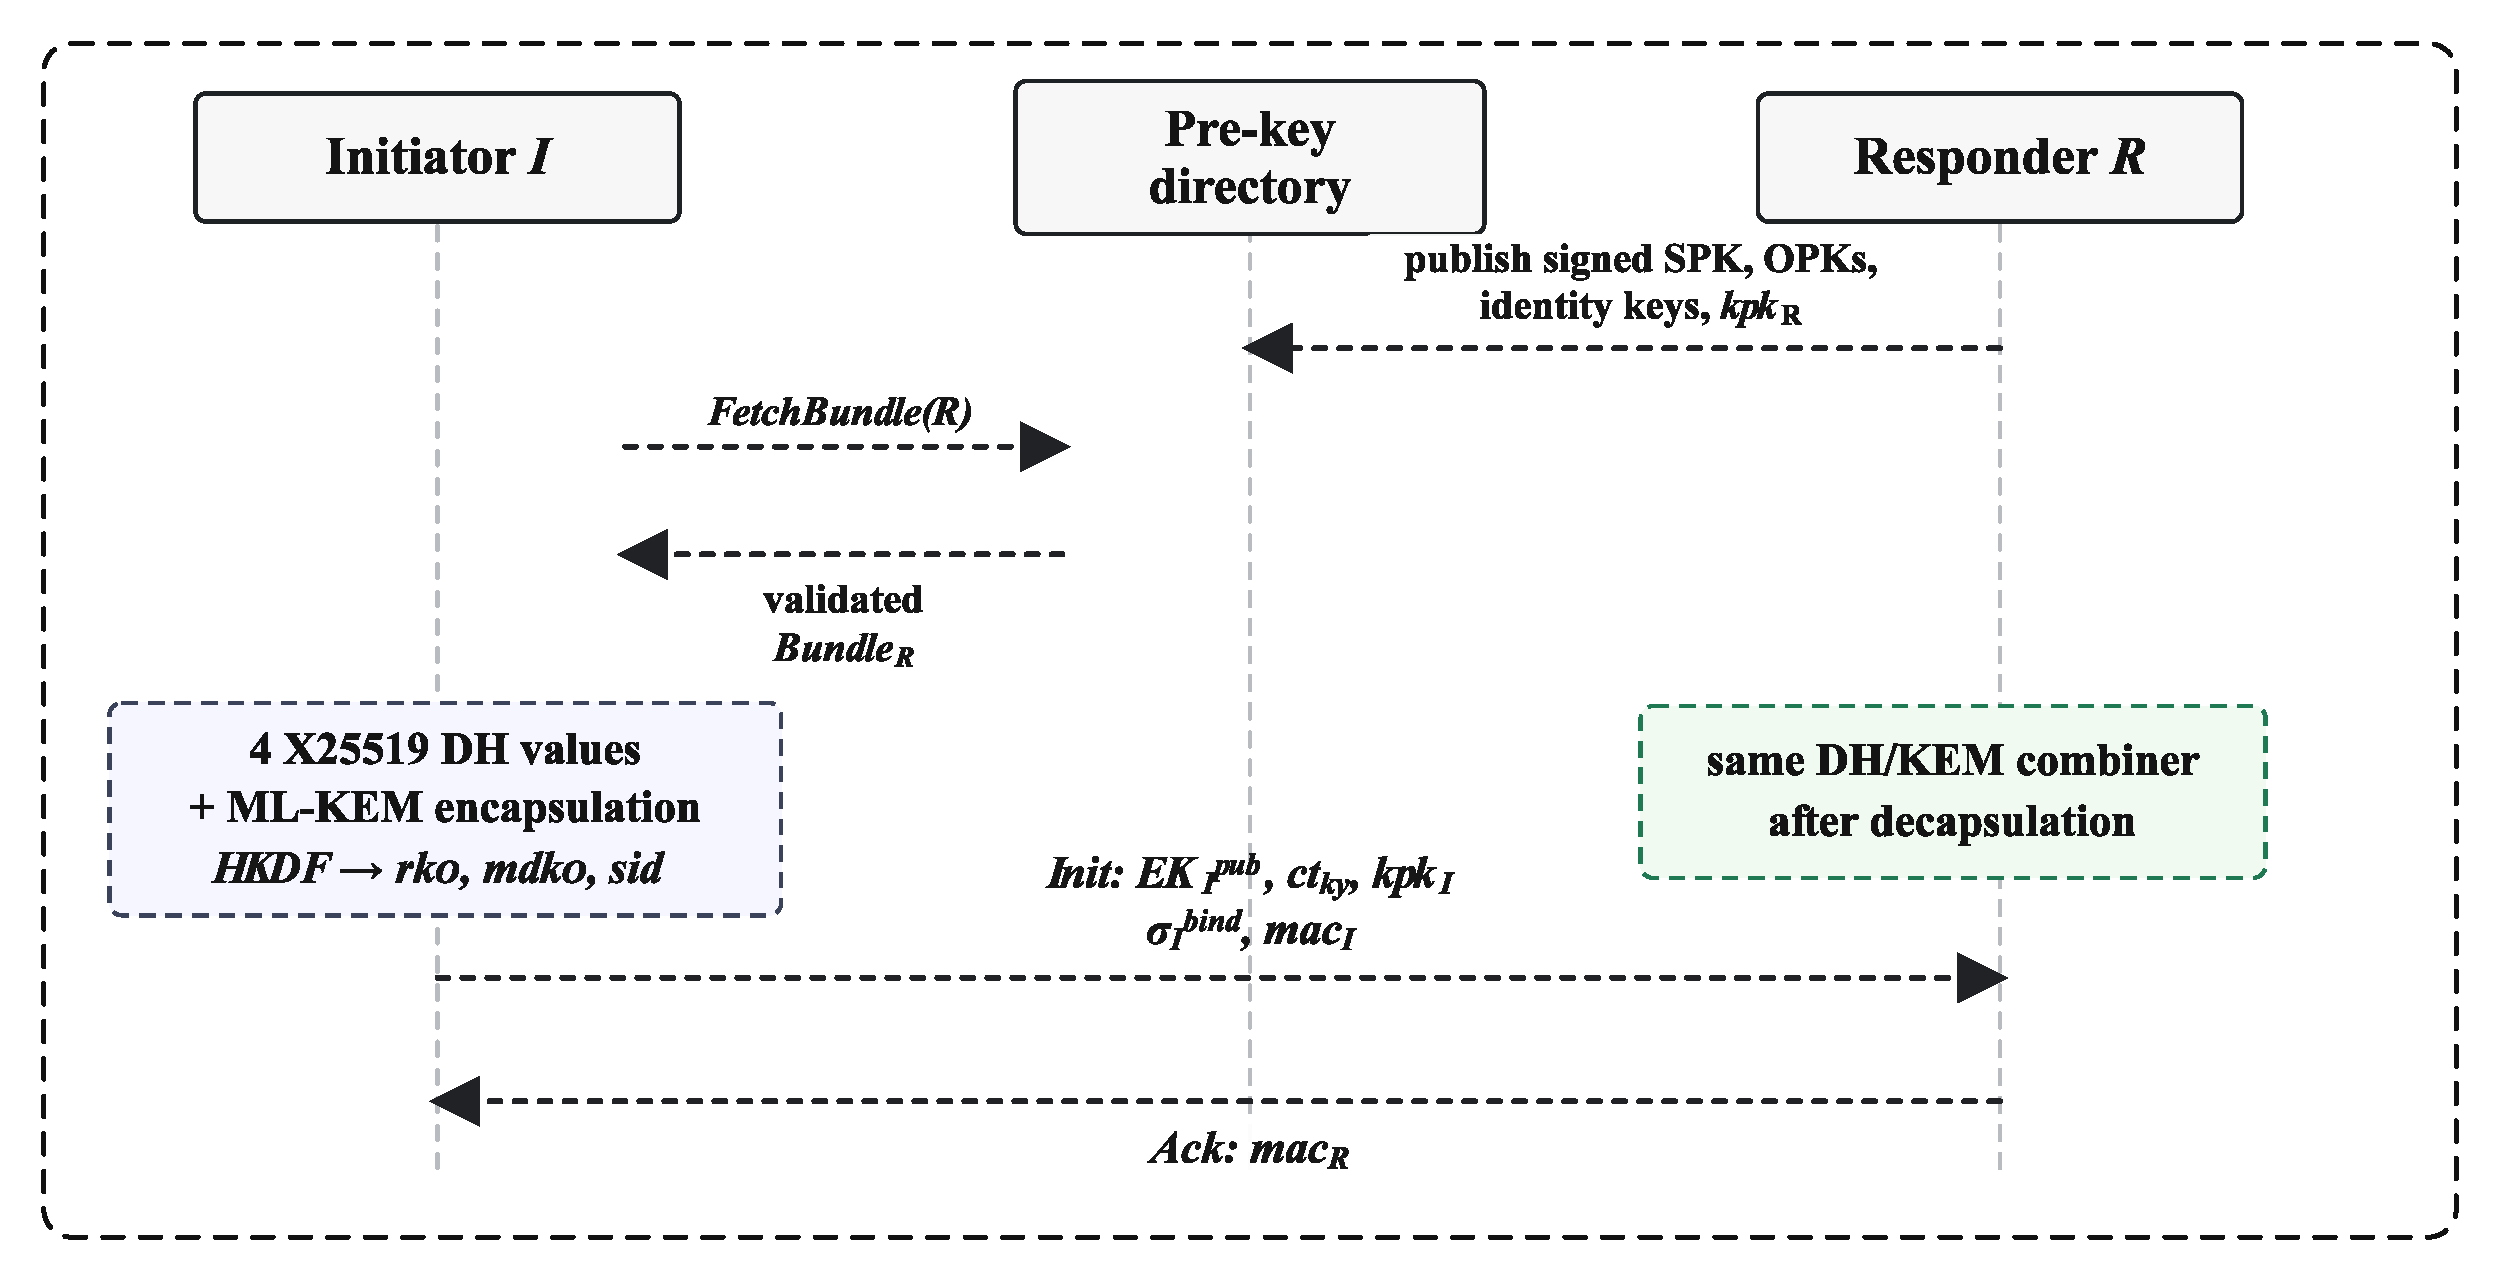
\includegraphics[width=0.98\textwidth]{figures/hybrid_x3dh_sequence_fixed.pdf}
\caption{Hybrid pre-key handshake messages and root-key inputs. The KEM public key is validated and transcript-bound by key confirmation. It is not a separate per-session signature.}\label{fig:handshake-flow}
\end{figure}

\begingroup
\LinesNotNumbered
\SetAlgoNoLine
\begin{algorithm}[tbp]
\caption{Initiator computation for the hybrid pre-key agreement.}\label{alg:initiator}
\footnotesize
\textbf{Inputs.}
Initiator identity $(ed_I,\IK_I)$, local KEM key $kpk_I$, and responder bundle $\mathit{Bundle}_R$.

\textbf{Outputs.}
Initial state $(\rk_0,\mdk_0,\mathit{sid})$ and $\mathit{Init}$ message.
\vspace{0.25\baselineskip}

\textbf{1. Validate responder material.}
Accept $\mathit{Bundle}_R$ only if the Ed25519 bindings verify, all X25519 public keys pass small-order rejection, and $kpk_R$ has a valid ML-KEM public-key encoding.

\textbf{2. Compute the classical pre-key contribution.}
Generate $(\mathit{ek}_I,\EK_I^{\mathit{pub}})$ and select $\OPK_R$ if present. Then compute
\[
\begin{aligned}
\mathit{dh}_1 &= \DH(\mathit{ik}_I,\SPK_R^{\mathit{pub}}),\\
\mathit{dh}_2 &= \DH(\mathit{ek}_I,\IK_R^{\mathit{pub}}),\\
\mathit{dh}_3 &= \DH(\mathit{ek}_I,\SPK_R^{\mathit{pub}}),\\
\mathit{dh}_4 &= \DH(\mathit{ek}_I,\OPK_R^{\mathit{pub}})\quad\text{if available},\\
\mathit{IKM} &= \mathrm{0xFF}^{32}\concat\mathit{dh}_1\concat\mathit{dh}_2\concat\mathit{dh}_3[\concat\mathit{dh}_4],\\
\mathit{cs} &= \HKDF(\mathit{IKM},32,\varepsilon,\domain{Aura-X3DH}).
\end{aligned}
\]

\textbf{3. Add the post-quantum contribution and derive session state.}
\[
\begin{aligned}
(\mathit{ct}_{\mathit{ky}},\mathit{ss}_{\mathit{ky}}) &\gets \KEM.\Encaps(kpk_R),\\
\rk_0 &\gets \HKDF(\mathit{ss}_{\mathit{ky}},32,\mathit{cs},\domain{Aura-Hybrid-X3DH}),\\
\mathit{sid} &\gets \HKDF(\rk_0,16,\mathit{ct}_{\mathit{ky}},\domain{Aura-SessionId}),\\
\mathit{ctx}_{\mathit{md}} &\gets
  \mathrm{sort}(\EK_I^{\mathit{pub}},\SPK_R^{\mathit{pub}})\concat\mathit{sid},\\
\mdk_0 &\gets \HKDF(\rk_0,32,\mathit{ctx}_{\mathit{md}},\domain{Aura-MetadataKey}),\\
\mathit{kc}_I &\gets \HKDF(\rk_0,32,\varepsilon,\domain{Aura-KeyConfirm-I}),\\
\mathit{kc}_R &\gets \HKDF(\rk_0,32,\varepsilon,\domain{Aura-KeyConfirm-R}).
\end{aligned}
\]

\textbf{4. Bind the initiator identity and transcript.}
\[
\begin{aligned}
m_I^{\mathit{bind}} &\gets
  \domain{Aura-Handshake-Init-Identity-Binding}
  \concat \mathit{ed}_I^{\mathit{pub}}\concat\IK_I^{\mathit{pub}}\concat kpk_I,\\
\sigma_I^{\mathit{bind}} &\gets
  \tech{Ed25519.Sign}(ed_I^{\mathit{sk}},m_I^{\mathit{bind}}),\\
\mathit{Init}_0 &\gets
  (\mathit{ed}_I^{\mathit{pub}},\IK_I^{\mathit{pub}},
  \EK_I^{\mathit{pub}},\mathit{ct}_{\mathit{ky}},kpk_I,\\
&\qquad \sigma_I^{\mathit{bind}},\mathit{opk\_id},N_{\max}),\\
\mathit{th} &\gets
  \HMAC(\domain{Aura-Handshake-Transcript},
  \mathsf{LP}(\mathit{Bundle}_R)\concat\mathsf{LP}(\mathit{Init}_0)),\\
\mathit{mac}_I &\gets \HMAC(\mathit{kc}_I,\mathit{th}),\\
\mathit{mac}_R^* &\gets \HMAC(\mathit{kc}_R,\mathit{th}),\\
\mathit{Init} &\gets(\mathit{Init}_0,\mathit{mac}_I).
\end{aligned}
\]
\end{algorithm}
\endgroup

Here $\mathsf{LP}(x)$ denotes the length-prefixed canonical encoding used by the transcript serializer.
Throughout the pseudocode, $\HKDF(\mathit{ikm},L,\mathit{salt},\mathit{info})$
means RFC~5869 Extract with $(\mathit{salt},\mathit{ikm})$ followed by Expand
to $L$ bytes with the stated $\mathit{info}$ string.
The initiator retains $\mathit{mac}_R^*$ for the responder acknowledgement and
keeps $\mathit{ss}_{\mathit{ky}}$ only in pending state for the initial
post-handshake ratchet. Ephemeral DH state and intermediate shared secrets are
erased after the derivation completes.

The responder performs the symmetric computation: it recomputes the four DH shared secrets using its own private keys, decapsulates the ML-KEM ciphertext, derives the same root key $\rk_0$, verifies $\mathit{mac}_I$, and sends $\mathit{Ack} = (\mathit{mac}_R)$. The initiator finalizes by verifying $\mathit{mac}_R$ in constant time.

\paragraph{Hybrid combiner design}
The combiner uses the classical DH output $\mathit{cs}$ as the HKDF salt and the ML-KEM shared secret $\mathit{ss}_{\mathit{ky}}$ as input keying material. This ordering follows the RFC~5869 interface~\cite{rfc5869}. Its robustness argument invokes the $\twoSourcePRF$ assumption in \cref{def:dual-prf}, not the ordinary extractor reading in which the salt is public and independent. If the classical reduction path applies, $\mathit{cs}$ supplies the fresh source. If the ML-KEM reduction path applies, $\mathit{ss}_{\mathit{ky}}$ supplies it. The construction therefore has two alternative security arguments, each conditioned on the exact HKDF assumption stated above.

\paragraph{Key confirmation}
Bilateral key confirmation prevents unknown key-share (UKS) attacks~\cite{lamacchia2007}. The transcript digest $\mathit{th}$ is computed with HMAC over length-prefixed inputs. Authentication is provided by the later HMAC under keys $\mathit{kc}_I$ and $\mathit{kc}_R$. These confirmation keys are derived from $\rk_0$ using distinct HKDF info strings, ensuring domain separation.

\paragraph{DH validation}
All received X25519 public keys are validated by checking against the eight small-order points of Curve25519 (points of order dividing the cofactor 8) using constant-time comparison to avoid data-dependent timing behavior. Additionally, points are verified to satisfy $\mathit{key} < p$ where $p = 2^{255} - 19$, using branchless word-by-word subtraction.

\subsection{Hybrid Double Ratchet}\label{sec:ratchet}

After the handshake, communication proceeds via the hybrid Double Ratchet, which combines a symmetric-key chain ratchet with an asymmetric hybrid ratchet.

\subsubsection{Symmetric Chain Ratchet}

Message keys are derived from the chain key via HKDF with distinct info strings for domain separation:
\begin{align}
  \mk_{e,n} &= \HKDF(\ck_e^{(n)},\, 32,\, \varepsilon,\, \domain{Aura-Msg}), \label{eq:msg-key} \\
  \ck_e^{(n+1)} &= \HKDF(\ck_e^{(n)},\, 32,\, \varepsilon,\, \domain{Aura-Chain}). \label{eq:chain-key}
\end{align}
The old chain key $\ck_e^{(n)}$ is securely erased after derivation, providing per-message forward secrecy within an epoch.

\subsubsection{Asymmetric Hybrid Ratchet}

\begingroup
\LinesNotNumbered
\SetAlgoNoLine
\begin{algorithm}[H]
\caption{Send-side hybrid ratchet transition (epoch $e \to e+1$).}\label{alg:send-ratchet}
\footnotesize
\textbf{Inputs.}
Current root key $\rk_e$ and peer ratchet public keys
$(D_{\mathit{peer}},kpk_{\mathit{peer}})$.

\textbf{Outputs.}
Updated sender state $(\rk_{e+1},\ck_{e+1},\mdk_{e+1}^{\mathit{send}})$ and
ratchet header $\mathit{Hdr}_{e+1}$.
\vspace{0.25\baselineskip}

\textbf{1. Generate fresh advertised sender material.}
\[
\begin{aligned}
(d_{e+1},D_{e+1}) &\gets \tech{X25519.KeyGen}(),\\
(kpk_{e+1},ksk_{e+1}) &\gets \KEM.\KeyGen().
\end{aligned}
\]

\textbf{2. Compute directed hybrid input material.}
\[
\begin{aligned}
\mathit{dh}_{e+1} &\gets \DH(d_{e+1},D_{\mathit{peer}}),\\
(\mathit{ct}_{e+1},\mathit{ss}_{e+1}) &\gets
  \KEM.\Encaps(kpk_{\mathit{peer}}),\\
\mathit{ikm}_{e+1} &\gets
  \mathit{dh}_{e+1}\concat\mathit{ss}_{e+1}.
\end{aligned}
\]

\textbf{3. Bind the next KEM public key into the KDF transcript.}
\[
\begin{aligned}
\mathit{info}_{e+1} &\gets
  \domain{Aura-Hybrid-Ratchet}\concat kpk_{e+1},\\
T_{e+1} &\gets
  \HKDF(\mathit{ikm}_{e+1},96,\rk_e,\mathit{info}_{e+1}),\\
(\rk_{e+1},\ck_{e+1},\mdk_{e+1}^{\mathit{send}}) &\gets
  \operatorname{split}_{32,32,32}(T_{e+1}).
\end{aligned}
\]

\textbf{4. Advertise the ratchet header.}
\[
\mathit{Hdr}_{e+1}\gets(D_{e+1},\mathit{ct}_{e+1},kpk_{e+1}).
\]
\end{algorithm}
\endgroup

The sender attaches $\mathit{Hdr}_{e+1}$ to the next envelope, installs the
new epoch state, and erases the previous DH/KEM private state, $\rk_e$,
$\mathit{dh}_{e+1}$, and $\mathit{ss}_{e+1}$ after derivation.
The recovery arguments for this transition use the $\splitInputPRF$
assumption in \cref{def:split-prf}, since only one component of
$\mathit{dh}_{e+1}\concat\mathit{ss}_{e+1}$ may remain secret.

\begin{figure}[H]
\centering
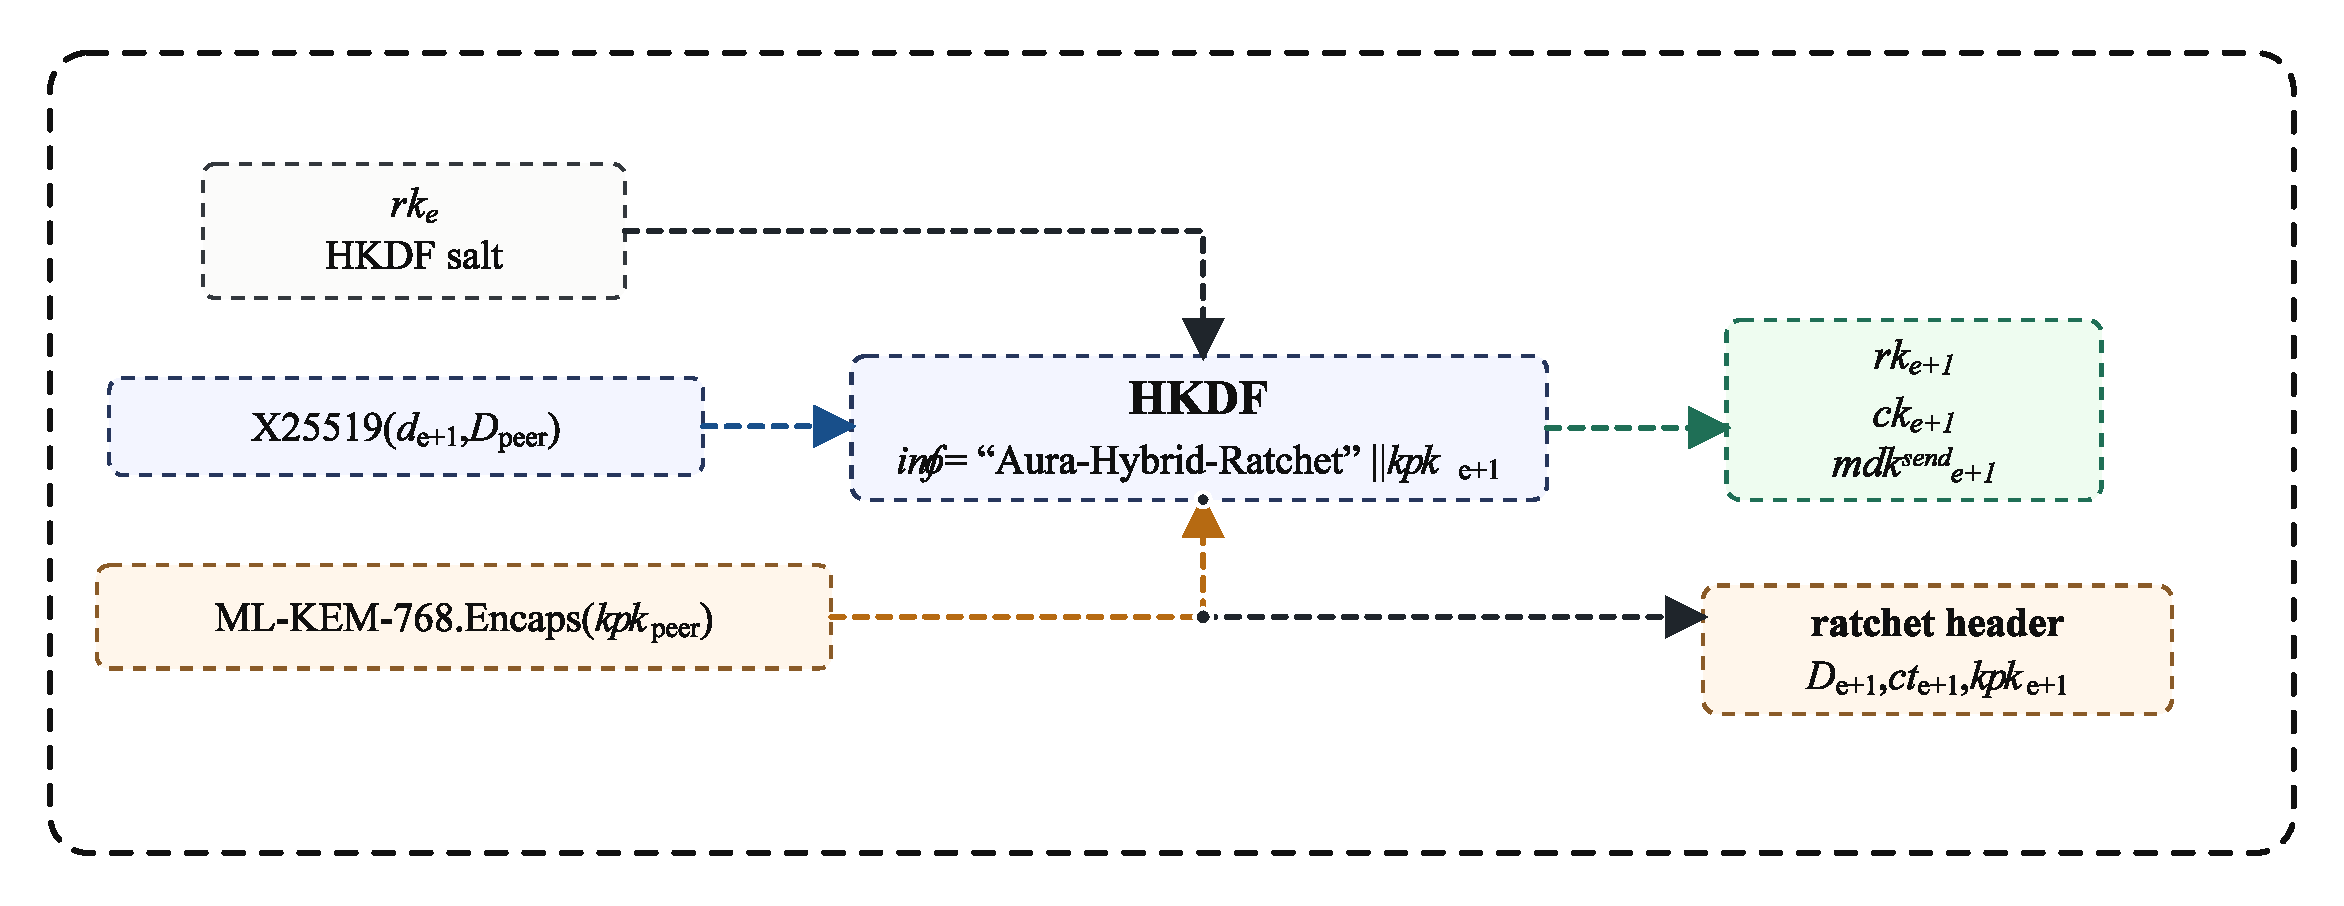
\includegraphics[width=0.98\textwidth]{figures/directed_hybrid_ratchet_step.pdf}
\caption{Send-side hybrid ratchet derivation and transmitted ratchet header. The new KEM public key is part of the HKDF info string, binding the advertised post-quantum state to the derived root.}\label{fig:ratchet-derivation}
\end{figure}

\paragraph{Ratchet trigger}
Classical DH ratchets normally advance the asymmetric step when a new peer DH
public key is received~\cite{signal-double-ratchet}. Aura Protocol uses a
single trigger rule for this directed hybrid design: after every received
message, the next outbound message executes a full X25519+ML-KEM ratchet and
advertises the resulting ratchet header. A chain-exhaustion ratchet is also
triggered when the negotiated per-chain limit $N_{\max}$ is reached.

\paragraph{Augmented info string}
The HKDF info parameter includes the new ML-KEM public key $kpk_{e+1}$ in \cref{alg:send-ratchet,fig:ratchet-derivation}. This binding supports the following lemma:

\begin{lemma}[Augmented HKDF Info Binding]\label{lem:augmented-hkdf}
If an adversary substitutes $kpk' \neq kpk_{e+1}$ in the ratchet header, the receiver's derived root key is computationally independent of the sender's root key, except with negligible HKDF-output collision probability. Consequently, all derived chain and message keys differ, and AEAD decryption fails under the $\INTCTXT$ property of $\AEAD$. This provides an implicit state-binding check for the KEM public key without per-step signatures. It does not provide a separate identity-authentication mechanism.
\end{lemma}

\begin{table}[H]
\centering
\caption{Operational traces for KEM public-key manipulation.}
\label{tab:kem-binding-traces}
\small
\begin{tabularx}{\textwidth}{@{}L{0.26\textwidth}L{0.33\textwidth}Y@{}}
\toprule
Adversarial action & Detection point & Security effect \\
\midrule
Substitute the responder's handshake KEM public key in the directory while keeping signed X25519 material unchanged. & The peers derive different handshake roots, so bilateral key-confirmation MACs do not validate. & The session is not established. This is denial of service, not a silent confidentiality downgrade. \\
Replace $kpk_{e+1}$ in a ratchet header. & The receiver uses $kpk'_{e+1}$ in HKDF info and derives a different root, chain key, and metadata key. Metadata or payload AEAD fails. & The candidate transition is rejected and the previous state is restored. \\
Replay an old ratchet header from the same session. & Epoch, nonce, replay-window, and cached-key checks are evaluated before candidate state is retained. & Admissible delayed traffic uses bounded compatibility state. Stale state-changing headers are rejected. \\
Omit or truncate KEM material to force a classical-only path. & Version, length, and profile checks fail before KDF input is accepted. & Hybrid policy enforcement prevents transparent fallback to a weaker transcript. \\
\bottomrule
\end{tabularx}
\end{table}

\paragraph{Receive-side ratchet}
The receiver evaluates a ratchet header against a temporary in-memory snapshot.
The candidate transition is retained only after syntactic validation, KEM
decapsulation, DH derivation, metadata and payload decryption, and replay checks
succeed. Durable export is a separate caller-controlled operation and is not
part of the decrypt call's atomic boundary.
The executable evidence for the pinned snapshot covers adversarial validation
and AEAD failures after candidate derivation; it does not claim atomic recovery
from arbitrary allocator, platform, or process failures.

\begingroup
\LinesNumbered
\SetAlgoLined
\begin{algorithm}[H]
\caption{Receive-side hybrid ratchet and transactional acceptance.}
\label{alg:receive-ratchet}
\footnotesize
\textbf{Inputs.}
Current state $S_e$, envelope $C$, optional ratchet header
$\mathit{Hdr}_{e+1}=(D_{e+1},ct_{e+1},kpk_{e+1})$.

\textbf{Outputs.}
Plaintext $M$ and committed state $S'$. On rejection, return $\bot$ and the
unchanged state $S_e$.
\vspace{0.25\baselineskip}

$S_{\mathit{old}}\gets S_e$\;
\If{$C$ has malformed version, length, epoch, or public-key fields}{
  \textbf{return} $(\bot,S_e)$\;
}
\If{$\mathit{Hdr}_{e+1}$ is present}{
  $\mathit{ss}_{e+1}\gets \KEM.\Decaps(ct_{e+1},ksk_e^{\mathit{local}})$\;
  $\mathit{dh}_{e+1}\gets \DH(d_e^{\mathit{local}},D_{e+1})$\;
  $\mathit{info}_{e+1}\gets \domain{Aura-Hybrid-Ratchet}\concat kpk_{e+1}$\;
  $T_{e+1}\gets \HKDF(\mathit{dh}_{e+1}\concat\mathit{ss}_{e+1},96,\rk_e,\mathit{info}_{e+1})$\;
  Install candidate $(\rk_{e+1},\ck_{e+1},\mdk_{e+1}^{\mathit{recv}})$ and cache old metadata keys for bounded delayed delivery\;
}
Derive or recover the candidate message key $\mk_{e,n}$ for the envelope epoch and index\;
\If{the nonce was already accepted or the replay window cannot represent it}{
  restore $S_{\mathit{old}}$ and \textbf{return} $(\bot,S_e)$\;
}
\If{metadata or payload AEAD decryption fails}{
  restore $S_{\mathit{old}}$ and \textbf{return} $(\bot,S_e)$\;
}
Commit replay state, skipped-key state, and root/chain/metadata keys in memory\;
Erase consumed DH, KEM, HKDF, and message-key material\;
\textbf{return} $(M,S')$\;
\end{algorithm}
\endgroup

\paragraph{Transactional rollback}
Before applying a received ratchet, the receiver records a temporary copy of the
current session state: root key, chain keys, DH/ML-KEM private keys, skipped
message keys, and metadata keys. If metadata or payload decryption fails after
the candidate ratchet is applied, the previous state is restored. A forged
ratchet envelope therefore cannot desynchronize the in-memory session. Crash
consistency and rollback freshness additionally require successful sealed-state
export and an external monotonic counter as described in \cref{sec:state}.

\begin{figure}[H]
\centering
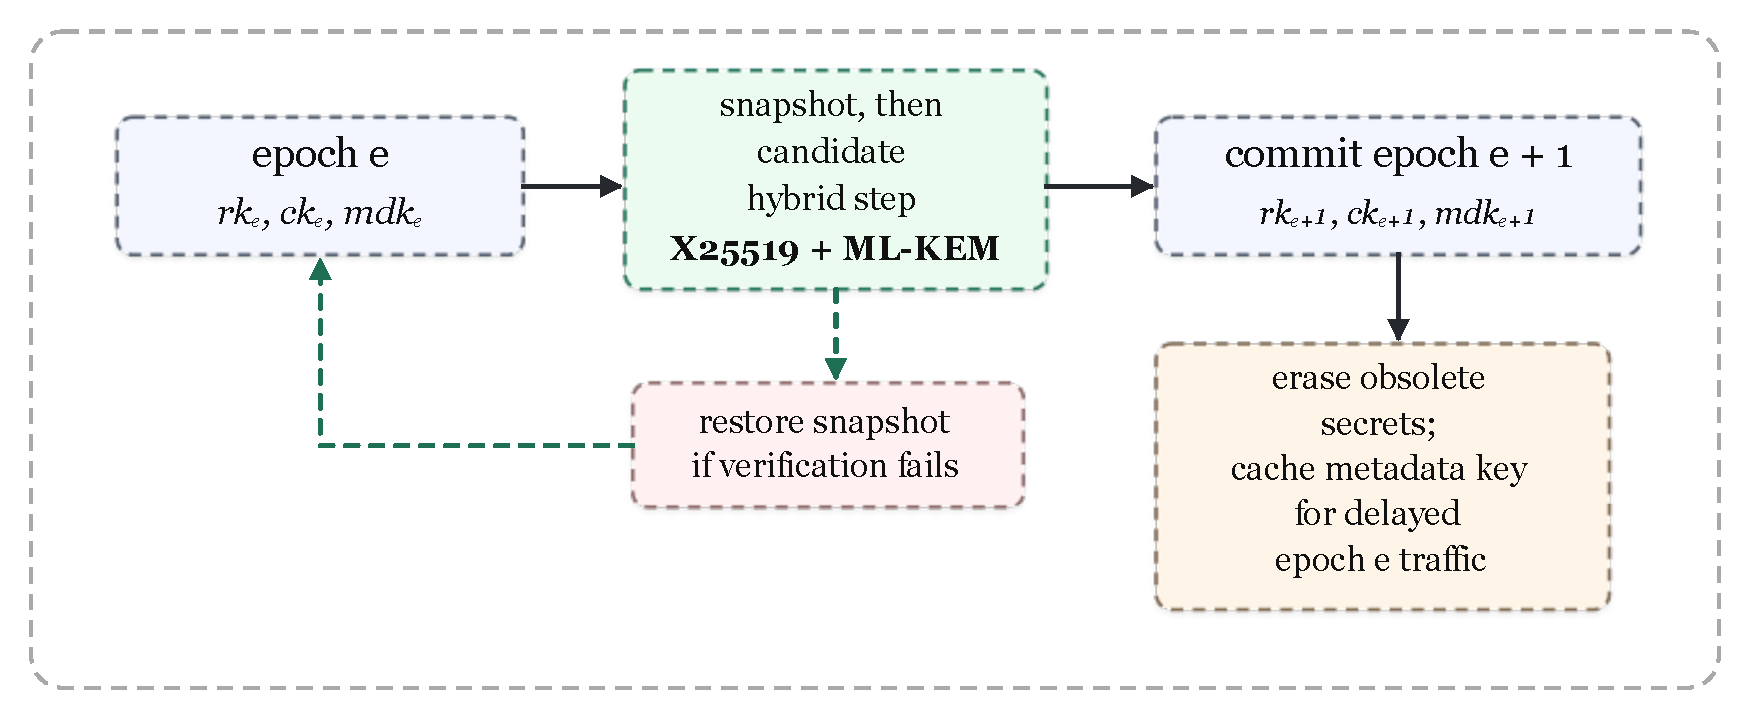
\includegraphics[width=0.92\textwidth]{figures/epoch_snapshot_hybrid_step.pdf}
\vspace{-0.25\baselineskip}
\caption{Ratchet state lifecycle. A successful hybrid step commits new root, chain, and metadata keys. Obsolete high-value secrets are erased after authentication, while bounded compatibility state is retained for delayed traffic and rollback safety.}\label{fig:ratchet-state-lifecycle}
\end{figure}

\subsubsection{Session Initialization}

After the hybrid pre-key handshake produces $\rk_0$ and the ML-KEM shared secret, the session is initialized via an initial hybrid ratchet step:
\begin{align}
  \mathit{dh}_{\mathit{init}} &= \DH(d_{\mathit{local}}, D_{\mathit{remote}}), \label{eq:init-dh} \\
  \mathit{hybrid\_ikm} &= \mathit{dh}_{\mathit{init}} \concat \mathit{ss}_{\mathit{ky}}, \label{eq:init-hybrid-ikm} \\
  T_{\mathit{init}} &= \HKDF(\mathit{hybrid\_ikm},\, 64,\, \rk_0,\, \domain{Aura-Hybrid-Ratchet}), \label{eq:init-transcript} \\
  \rk_1 &= T_{\mathit{init}}[0{:}32], \label{eq:init-root-key} \\
  (\ck_{\mathit{send}},\, \ck_{\mathit{recv}}) &= \HKDF(\rk_1,\, 64,\, \varepsilon,\, \domain{Aura-ChainInit}). \label{eq:init-chain-keys}
\end{align}
The final post-handshake root used by the message layer is $\rk_1$. The value $\mdk_0$ remains the initial metadata key until the first ratchet. The initiator uses the first 32 bytes of the \domain{Aura-ChainInit} output as $\ck_{\mathit{send}}$ and the last 32 bytes as $\ck_{\mathit{recv}}$. The responder swaps them. The AKE claim establishes pseudorandomness of $\rk_0$. Post-handshake initialization carries this property to $(\rk_1,\ck_{\mathit{send}},\ck_{\mathit{recv}})$ through HKDF domain separation with $\rk_0$ as salt.

\subsection{Two-Layer AEAD Encryption}\label{sec:two-layer}

Each message envelope consists of two independently encrypted layers:

\paragraph{Layer 1: Metadata}
\begin{equation}\label{eq:metadata-aead}
  \mathit{ct}_{\mathit{md}} = \AEAD.\Enc(\mdk_e^{\mathit{send}},\, \mathit{nonce}_{\mathit{md}},\, \mathit{metadata},\, \mathit{aad}_{\mathit{md}}),
\end{equation}
where $\mathit{aad}_{\mathit{md}} = \mathit{sid} \concat \mathit{ibh} \concat \epoch \concat v$ includes the session ID, identity binding hash, epoch counter, and protocol version. The metadata contains the message index, payload nonce, envelope type, and correlation identifiers.

\paragraph{Layer 2: Payload}
\begin{equation}\label{eq:payload-aead}
  \mathit{ct}_{\mathit{pay}} = \AEAD.\Enc(\mk_{e,n},\, \mathit{nonce}_{\mathit{pay}},\, \mathit{plaintext},\, \mathit{aad}_{\mathit{pay}}),
\end{equation}
where $\mathit{aad}_{\mathit{pay}} = \mathit{sid} \concat \mathit{ibh} \concat \epoch \concat n \concat v$ additionally includes the message index $n$.

\begin{figure}[H]
\centering
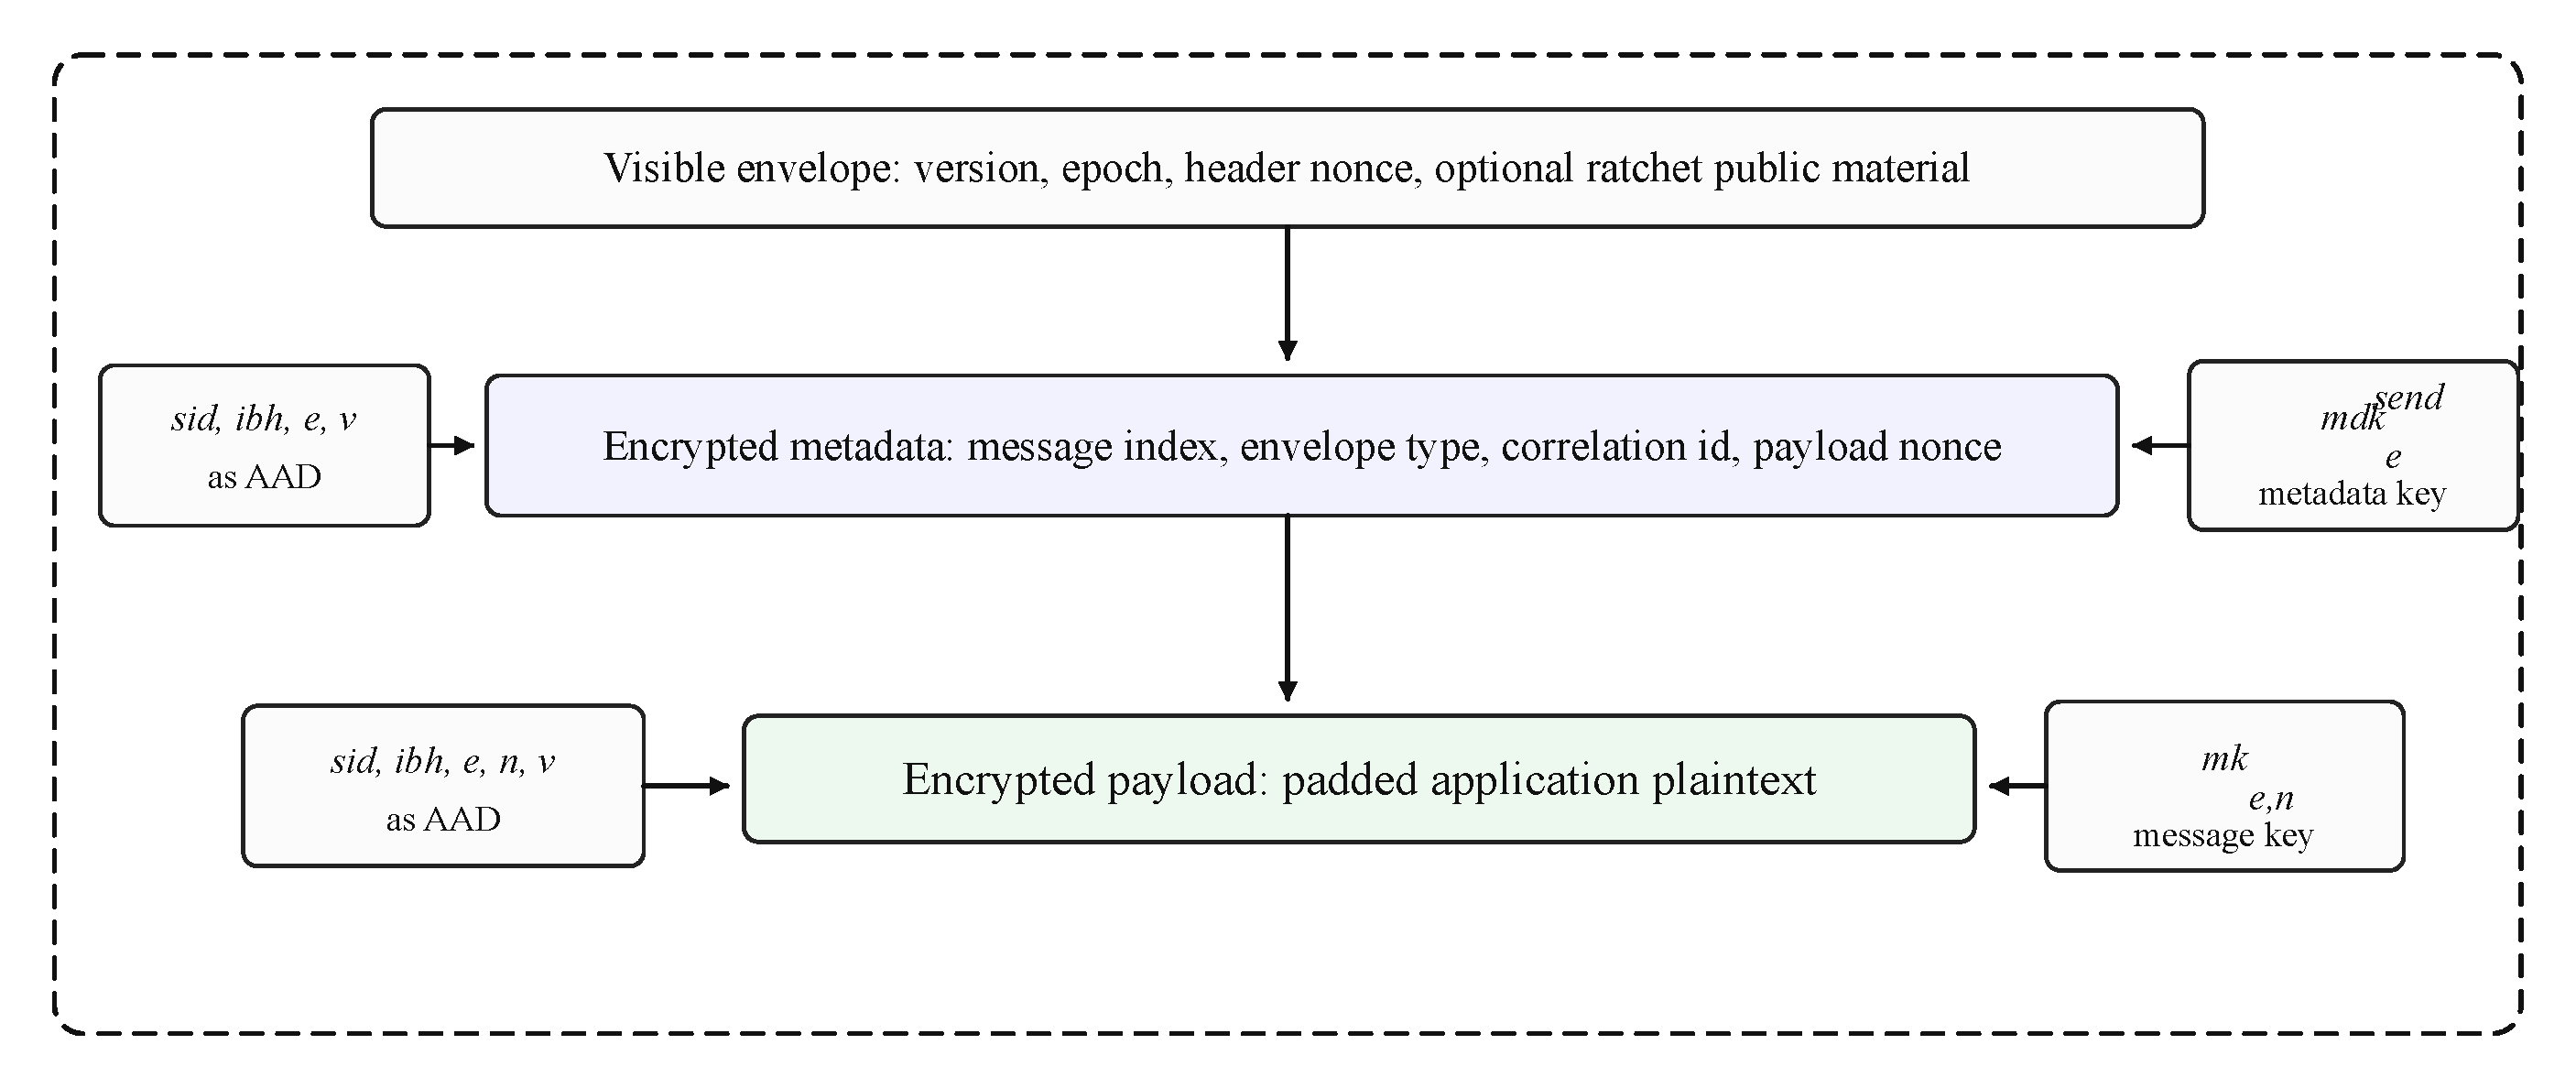
\includegraphics[width=0.98\textwidth]{figures/secure_message_packaging_flowchart_fixed_v2.pdf}
\vspace{-0.25\baselineskip}
\caption{Envelope protection split: visible transport fields, encrypted metadata, and encrypted payload. Delivery timing, sizes, and ratchet public material remain visible. Sender metadata and application content are protected by separate AEAD keys.}\label{fig:two-layer-envelope}
\end{figure}

\begin{table}[H]
\centering
\caption{Metadata-confidentiality boundary of the two-layer envelope.}
\label{tab:metadata-boundary}
\small
\begin{tabularx}{\textwidth}{@{}L{0.22\textwidth}L{0.36\textwidth}Y@{}}
\toprule
Class & Examples & Protection statement \\
\midrule
Protected by the metadata AEAD & Message index, payload nonce, envelope type, application correlation identifiers. & Confidential and integrity-protected under the per-epoch metadata key $\mdk_e$, with session, identity, epoch, and version bound as AAD. \\
Protected by the payload AEAD & Application plaintext and application-level confidential content. & Confidential and integrity-protected under per-message keys $\mk_{e,n}$ derived from the chain key. \\
Partially observable through traffic shape & Direction changes, burst structure, retries, and approximate conversation activity. & Not directly encoded in plaintext fields, but may be inferred from header presence, ciphertext lengths, and delivery behavior. \\
Visible by design & Protocol version, total frame length, delivery timing, transport endpoints, ratchet DH public key, ML-KEM ciphertext, and advertised KEM public key. & Required for routing or state synchronization. These fields are outside the metadata-confidentiality claim and are left to transport padding, sender-hiding delivery, or anonymity systems. \\
\bottomrule
\end{tabularx}
\end{table}

\begin{lemma}[Two-Layer AEAD Independence]\label{lem:two-layer}
For a ratchet epoch, the chain key $\ck_e$ and metadata key $\mdk_e$ are disjoint segments of a jointly pseudorandom HKDF output. The payload message key $\mk_{e,n}$ is later derived from $\ck_e$ under the \domain{Aura-Msg} domain label. Given only $\mk_{e,n}$ and not the root or metadata key material, the adversary obtains no information about $\mdk_e$ under the HKDF PRF assumption and the one-way chain derivation.
\end{lemma}

\paragraph{Nonce structure}
Payload nonces use a structured 12-byte layout:
\begin{equation}\label{eq:nonce-layout}
  \mathit{nonce} =
  \mathit{prefix}[8] \concat
  \mathit{counter}_{\mathrm{LE}}[2] \concat
  \mathit{msg\_index}_{\mathrm{LE}}[2].
\end{equation}
The prefix is sampled by the CSPRNG when the send nonce generator is created
or reset at a ratchet boundary, the counter is monotonically increasing,
and the message index provides per-chain addressability. Metadata encryption
uses an independent random 12-byte header nonce. A ratchet is required before
the negotiated message-chain limit is exceeded or either 16-bit field is
exhausted. The construction also exposes a nonce-budget warning threshold for
operational monitoring.

\paragraph{Identity binding hash}
Every AEAD additional-data construction includes an identity binding hash:
\begin{equation}\label{eq:identity-binding}
  \begin{aligned}
  \mathit{ibh} = \SHA(&\domain{Aura-Identity-Binding} \concat
  \mathrm{sort}(\mathit{ed}^{\mathit{pub}}_I,
    \mathit{ed}^{\mathit{pub}}_R)\\
  &\concat
  \mathrm{sort}(\IK^{\mathit{pub}}_I,\IK^{\mathit{pub}}_R)).
  \end{aligned}
\end{equation}
where both Ed25519 and X25519 public key pairs are lexicographically sorted before concatenation. This binds AEAD data to the unordered pair of identities. Role separation is provided by the handshake transcript, key-confirmation direction labels, and initiator/responder chain-key assignment.

\subsection{Replay Protection}\label{sec:replay}

Replay protection is achieved through a bounded nonce cache:
\begin{itemize}
  \item A $\mathsf{HashSet}$ of seen payload nonces, bounded to $W = 2{,}048$ entries.
  \item Nonces embed a monotonic counter in bytes $[8{:}10]$. When the cache is full, the oldest observed nonce entries are evicted first.
  \item Duplicate nonces are immediately rejected before payload decryption.
\end{itemize}

\subsection{State Persistence}\label{sec:state}

Session state is serialized via Protocol Buffers and protected by two mechanisms:
\begin{itemize}
  \item \textbf{State integrity HMAC:} An HMAC-SHA256 tag computed over the serialized state (key derived from the root key via $\HKDF$) authenticates serialized-state integrity. Rollback freshness requires the external monotonic counter used by sealed-state import/export.
  \item \textbf{Sealed export:} For persistent storage, the state is encrypted using a double-envelope construction: a random data encryption key (DEK) encrypts the state, and the DEK is encrypted under a caller-provided key encryption key (KEK), both using $\AEAD$.
\end{itemize}


% ═════════════════════════════════════════════════════════════
% 5. SECURITY MODEL
% ═════════════════════════════════════════════════════════════
\section{Security Model}\label{sec:security-model}

The security model is inspired by the $\eCK$ family of AKE models~\cite{canetti2001,lamacchia2007} and adapted to the hybrid post-quantum setting. Its oracle and freshness rules differ from standard eCK formulations. The claims below therefore apply only to the model defined here.

\begin{definition}[Parties and Sessions]\label{def:parties}
There are at most $N$ parties, each holding an X25519 identity keypair $\IK_i$, an Ed25519 signing keypair, an ML-KEM-768 keypair $(kpk_i, ksk_i)$, rotating signed pre-keys, and one-time pre-keys. A session $\pi_i^s$ denotes a protocol run by party $P_i$ with intended partner $P_j$.
\end{definition}

\begin{definition}[Adversary Oracles]\label{def:oracles}
The adversary $\advA$ has access to the following oracles:
\begin{itemize}
  \item $\textsf{Send}(\pi_i^s, m)$: Deliver message $m$ to session $\pi_i^s$ and obtain the response.
  \item $\textsf{Corrupt}(P_i)$: Obtain all long-term keys of $P_i$ ($\mathit{ik}_i$, Ed25519 signing key, $ksk_i$).
  \item $\textsf{RevealSPK}(P_i,\mathit{spk\_id})$: Obtain the private scalar for a selected signed pre-key.
  \item $\textsf{RevealOPK}(P_i,\mathit{opk\_id})$: Obtain the private scalar for an unused one-time pre-key. Consumed OPKs are modeled as deleted.
  \item $\textsf{RevealState}(\pi_i^s)$: Obtain the full session state (root key, chain keys, metadata keys, DH/ML-KEM private keys, nonce state).
  \item $\textsf{RevealSessionKey}(\pi_i^s)$: Obtain the current root key $\rk_e$.
  \item $\textsf{Test}(\pi_i^s)$: Challenge oracle. Flip coin $b \getsr \{0,1\}$. Return $\rk_e$ if $b = 0$ and a uniformly random key if $b = 1$. At most one $\textsf{Test}$ query is allowed.
\end{itemize}
\end{definition}

\begin{definition}[Partnering]
Sessions $\pi_i^s$ and $\pi_j^t$ are \emph{partnered} if they share the same transcript hash $\mathit{th}$.
\end{definition}

\begin{definition}[Freshness]\label{def:freshness}
A session $\pi_i^s$ with partner $\pi_j^t$ is \emph{fresh} if the adversary has not:
\begin{enumerate}
  \item Queried $\textsf{RevealSessionKey}$ or $\textsf{RevealState}$ on either $\pi_i^s$ or $\pi_j^t$ before $\textsf{Test}$.
  \item Queried both $\textsf{Corrupt}(P_i)$ and $\textsf{RevealState}(\pi_i^s)$ before the tested session completed.
  \item Queried $\textsf{Corrupt}(P_j)$ before session $\pi_j^t$ was created and no OPK was used.
  \item Queried $\textsf{RevealSPK}(P_j,\mathit{spk\_id})$ for the responder signed pre-key used in the tested session before $\textsf{Test}$ and no OPK was used and deleted.
  \item Queried $\textsf{RevealOPK}(P_j,\mathit{opk\_id})$ for the OPK used in the tested session before it was consumed.
\end{enumerate}
\end{definition}

\begin{definition}[Aura AKE Security]\label{def:ake}
Aura Protocol is secure in the model above if for all $\ppt$ adversaries $\advA$:
\begin{equation}\label{eq:eck-advantage}
  \adv^{\AKE}_{\mathrm{AURA}}(\advA) = \left|\Pr[\advA \text{ wins}] - \frac{1}{2}\right| \leq \negl(\secpar),
\end{equation}
where $\advA$ wins by correctly guessing $b$ for a fresh tested session.
This game measures key indistinguishability for fresh partnered sessions. The
correspondence properties used for peer authentication are stated separately.
\end{definition}

\begin{definition}[Forward Secrecy]\label{def:fs}
If an adversary learns the parties' long-term identity keys and
long-term KEM decapsulation keys at time $t$, the adversary still
cannot decrypt messages sent before $t$ in sessions whose key agreement
completed before the compromise. This claim requires that either the
responder signed-pre-key private scalar remains undisclosed or a
consumed OPK private scalar was used and deleted.
\end{definition}

\begin{definition}[Post-Compromise Security~\cite{cohn-gordon2020}]\label{def:pcs}
After full state compromise at epoch $e$ via $\textsf{RevealState}$, messages at epoch $\geq e + k$ are secure, provided the adversary does not compromise new keys generated after epoch $e$. The analysis distinguishes $k = 1$ (classical PCS) from $k = 2$ (hybrid PCS).
\end{definition}


% ═════════════════════════════════════════════════════════════
% 6. SECURITY ANALYSIS
% ═════════════════════════════════════════════════════════════
\section{Security Analysis}\label{sec:proofs}

This section gives six reduction-style security claims for Aura Protocol. Each
claim is accompanied by an argument sketch in the custom model of
\cref{sec:security-model}. These sketches identify the relevant assumptions and
loss terms, but they are not substitutes for complete game-by-game reductions.

\subsection{Hybrid Root-Key Pseudorandomness}\label{sec:thm1}

\begin{securityclaim}[Hybrid Root-Key Pseudorandomness]\label{thm:hybrid-combiner}
If $\KEM$ is $\INDCCA$ secure \textbf{or} $\DH$ satisfies $\GapCDH$ in the $\ROM$, then the Aura Protocol hybrid combiner
\begin{equation}\label{eq:combiner-root}
  \rk_0 =
  \HKDF(\mathit{ss}_{\mathit{ky}},\, 32,\,
  \mathit{cs},\, \domain{Aura-Hybrid-X3DH})
\end{equation}
outputs a pseudorandom root key under the additional assumption in
\cref{def:dual-prf}. The argument gives two alternative
reduction paths:
\begin{align}
  \begin{aligned}
  \adv^{\mathsf{rk}}_{\mathrm{Hybrid}}(\advA)
  &\leq
    \adv^{\INDCCA}_{\KEM}(\advB_1)
    + \adv^{\twoSourcePRF}_{\HKDF}(\advB_3)
    + \frac{q_H}{2^{256}},
  \end{aligned}
  \label{eq:combiner-bound-kem}\\
  \begin{aligned}
  \adv^{\mathsf{rk}}_{\mathrm{Hybrid}}(\advA)
  &\leq
    4 \cdot \adv^{\GapCDH}_{\DH}(\advB_2)
    + \adv^{\twoSourcePRF}_{\HKDF}(\advB_3)
    + \frac{q_H}{2^{256}}.
  \end{aligned}
  \label{eq:combiner-bound-dh}
\end{align}
where $q_H$ is the number of random-oracle queries. The classical path models
the inner \domain{Aura-X3DH} extraction in the random-oracle model. The factor 4
accounts for selecting the DH term used by that path.
\end{securityclaim}

\begin{proof}[Argument sketch]
There are two reduction paths. In the KEM path, the argument replaces the ML-KEM shared
secret $\mathit{ss}_{\mathit{ky}}$ with a uniformly random value, reducing
the distinguishing advantage to $\adv^{\INDCCA}_{\KEM}(\advB_1)$. In the
classical path, it replaces the classical pre-key shared secret $\mathit{cs}$ with a random
value via the $\GapCDH$ oracle. The factor~4 accounts for selecting one of the
four DH pairs $\mathit{dh}_1, \ldots, \mathit{dh}_4$. Either path leaves at
least one HKDF input uniformly random, so the $\twoSourcePRF$
property makes $\rk_0$ indistinguishable from random. The two cases give
\cref{eq:combiner-bound-kem,eq:combiner-bound-dh}. The $q_H/2^{256}$ term
bounds random oracle collisions.
\end{proof}

\subsection{AKE Security}

\begin{securityclaim}[AKE Security in the Modified Pre-Key Leakage Model]\label{thm:ake}
Aura Protocol's hybrid pre-key agreement satisfies the AKE security definition above. For any
$\ppt$ adversary $\advA$ making at most $q_s$ session queries, define the two
alternative combiner-path losses
\begin{align*}
  \Delta_{\mathsf{KEM}}
  &= \adv^{\INDCCA}_{\KEM}(\advB_2)
     + \adv^{\twoSourcePRF}_{\HKDF}(\advB_3),\\
  \Delta_{\mathsf{DH}}
  &= 4\cdot\adv^{\GapCDH}_{\DH}(\advB_1)
     + \adv^{\twoSourcePRF}_{\HKDF}(\advB_3).
\end{align*}
For either $X\in\{\mathsf{KEM},\mathsf{DH}\}$ whose assumptions hold, the
corresponding reduction path gives
\begin{align}
  \adv^{\AKE}_{\mathrm{AURA}}(\advA)
  &\leq q_s \cdot \Bigl(
    \Delta_X + 2 \cdot \adv^{\PRF}_{\HMAC}(\advB_4) \notag\\
  &\qquad
    + 3 \cdot \adv^{\SUFCMA}_{\mathrm{Ed25519}}(\advB_5)\Bigr)
    + \frac{q_s^2}{2^{128}} + \frac{q_H}{2^{256}}. \label{eq:ake-bound}
\end{align}
No minimum of the two reduction advantages is asserted.
\end{securityclaim}

\begin{proof}[Argument sketch]
The reduction guesses the tested session, losing a factor $q_s$. It then uses
one of the two combiner paths in \cref{thm:hybrid-combiner}: either replace the
ML-KEM shared secret by random, or replace the surviving pre-key DH contribution by
random. HKDF then yields a pseudorandom root key through the $\twoSourcePRF$
property. Finally, the reduction replaces the key-confirmation MACs with random
tags, reducing to $\PRF$ security of $\HMAC$. The factor~2 accounts for
$\mathit{mac}_I$ and $\mathit{mac}_R$. A successful identity or pre-key
substitution must forge one of the initiator identity-binding, responder
identity-binding, or responder signed-pre-key signatures. This gives the three
$\SUFCMA$ terms. The term $q_s^2/2^{128}$ bounds 128-bit session ID collisions.
The signature term is classical. The claim does not provide post-quantum active
authentication once Ed25519 is broken.
\end{proof}

\begin{lemma}[Bilateral Key Confirmation Prevents UKS]\label{lem:key-confirm}
Assume that the parties begin with verified identity keys and use the canonical
transcript encoding. An adversary who does not know $\rk_0$ cannot forge a valid
key-confirmation MAC. The keys $\mathit{kc}_I$ and $\mathit{kc}_R$ are derived
from $\rk_0$ under distinct HKDF labels, and each MAC covers the transcript hash
that binds both identities and the ephemeral key material.
\end{lemma}

\begin{lemma}[Domain Separation]\label{lem:domain-sep}
Let $\mathcal{L}_{\HKDF}$ be the set of labels used as HKDF info strings in
the construction. The labels in $\mathcal{L}_{\HKDF}$ are pairwise distinct
and are disjoint from labels used for transcript hashing, identity binding,
signatures, and auxiliary validation paths. Thus distinct HKDF invocations are
modeled as distinct oracle inputs in the $\ROM$ and as distinct PRF inputs in
the standard-model analysis.
\end{lemma}

\subsection{Forward Secrecy}

\begin{securityclaim}[Forward Secrecy]\label{thm:fs}
For any $\ppt$ adversary $\advA$ who obtains the long-term identity and KEM keys at time $t$, and for sessions whose responder signed-pre-key private scalar remains undisclosed or whose consumed OPK private scalar has already been deleted:
\begin{equation}\label{eq:fs-bound}
  \adv^{\mathrm{FS}}_{\mathrm{AURA}}(\advA) \leq \adv^{\GapCDH}_{\DH}(\advB_1) + \adv^{\twoSourcePRF}_{\HKDF}(\advB_2).
\end{equation}
This is a classical forward-secrecy bound under later disclosure of long-term
KEM secret keys. If both the responder SPK private scalar and KEM secret key
are later disclosed, and no deleted OPK contributed to the transcript, this
classical FS claim does not apply. The initial KEM ciphertext gives
harvest-now-decrypt-later protection only while the corresponding KEM secret
key is not later disclosed.
This is a fixed-session bound. A multi-session game incurs the corresponding
session-selection loss.
\end{securityclaim}

\begin{proof}[Argument sketch]
In the first hybrid transition, security comes from a DH term whose private scalar is unavailable
after compromise: $\mathit{dh}_3$ if the responder SPK private scalar is not
revealed, or $\mathit{dh}_4$ if a consumed OPK was used and deleted. The
transcript-visible term $\mathit{dh}_2=\DH(\mathit{ek}_I,\IK_R^{\mathit{pub}})$
is not counted after $\mathit{ik}_R$ disclosure, because it can be recomputed
from $\IK_R$ and $\EK_I^{\mathit{pub}}$. The surviving classical shared secret
is used as the HKDF salt, so the $\twoSourcePRF$ property makes the root key
pseudorandom. The initial KEM term is intentionally not counted in this FS bound:
after later disclosure of $\mathit{ksk}_R$, a recorded KEM ciphertext can be
decapsulated. The KEM contribution in this setting is HNDL protection without
later KEM secret-key disclosure, and PCS after fresh ratchet KEM keys appear.
\end{proof}

\begin{lemma}[Ephemeral Key Erasure]\label{lem:erasure}
Temporary DH outputs, KEM shared secrets, and intermediate key-derivation
buffers are assumed to be erased immediately after the derivation that consumes
them. A ratchet private key that remains part of the live session state is not
treated as erased until a later ratchet transition replaces it. The
implementation evidence in \cref{sec:implementation} addresses this erasure
assumption at the level of executable state management.
\end{lemma}

\subsection{Post-Compromise Security}\label{sec:thm-pcs}

\begin{figure}[H]
\centering
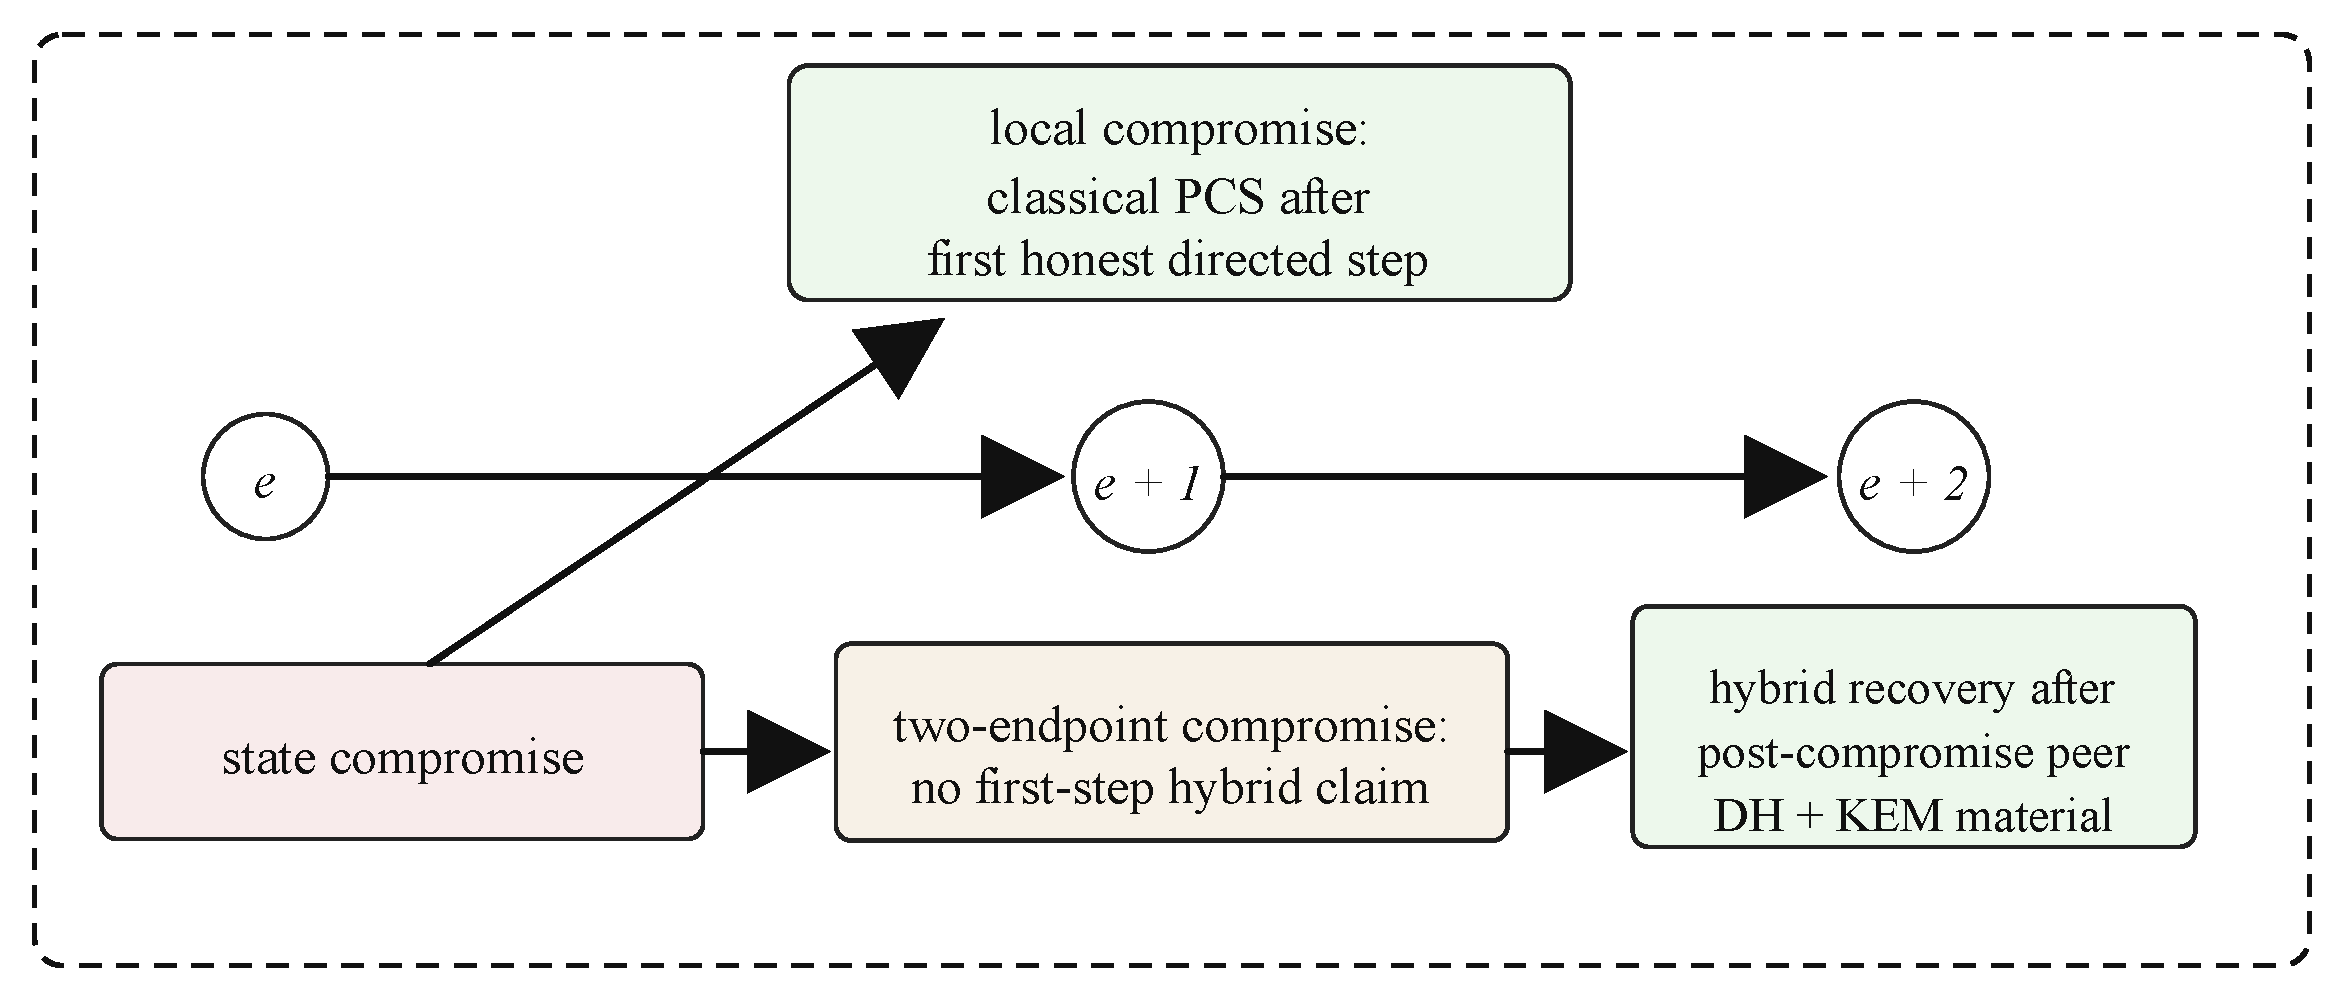
\includegraphics[width=0.98\textwidth]{figures/compromise_epochs_fixed_v3.pdf}
\vspace{-0.25\baselineskip}
\caption{Recovery conditions for local versus two-endpoint state compromise. Recovery requires a later honest directed ratchet step.}\label{fig:pcs-timeline}
\end{figure}

\begin{securityclaim}[Post-Compromise Security]\label{thm:pcs}
If the adversary compromises session state at epoch $e$ via
$\textsf{RevealState}$ and then stops learning post-compromise secrets:

\noindent\textbf{(a) Local classical PCS (1-step):} If the compromise is local to the sender endpoint, or more generally the peer DH private scalar used by the next directed DH remains undisclosed, messages after the first honest directed ratchet step are secure:
\begin{equation}\label{eq:pcs-classical-bound}
  \adv^{\mathrm{PCS}\text{-}1}_{\mathrm{AURA}}(\advA) \leq \adv^{\GapCDH}_{\DH}(\advB_1) + \adv^{\splitInputPRF}_{\HKDF}(\advB_2).
\end{equation}

\noindent\textbf{(b) Two-endpoint hybrid recovery:} If both endpoints' epoch-$e$ DH and KEM ratchet secrets are exposed, no first-step PCS is claimed. Messages after the next directed step that uses post-compromise peer DH and KEM public keys are secure. The DH and KEM reduction paths respectively give
\begin{align}
  \adv^{\mathrm{PCS}\text{-}2}_{\mathrm{AURA}}(\advA)
  &\leq \adv^{\GapCDH}_{\DH}(\advB_1)
  + \adv^{\splitInputPRF}_{\HKDF}(\advB_2),
  \label{eq:pcs-hybrid-bound-dh}\\
  \adv^{\mathrm{PCS}\text{-}2}_{\mathrm{AURA}}(\advA)
  &\leq \adv^{\INDCCA}_{\KEM}(\advB_3)
  + \adv^{\splitInputPRF}_{\HKDF}(\advB_2).
  \label{eq:pcs-hybrid-bound-kem}
\end{align}
These are fixed-transition bounds. A game in which the reduction must select one
transition among many adds the corresponding selection loss.
\end{securityclaim}

\begin{proof}[Argument sketch]\renewcommand{\qedsymbol}{}
The key subtlety is that the first post-compromise directed step uses the
peer's epoch-$e$ DH and KEM public keys. If the corresponding peer DH private
scalar was also revealed, the adversary can compute that first DH contribution
from the sender's new public key. The claim therefore separates local
state compromise from true two-endpoint state compromise.

\textbf{Part (a):} At the first honest directed step, the honest party generates a fresh DH keypair $(d_{e+1}, D_{e+1})$ unknown to the adversary. If the peer DH private scalar for $D_{\mathit{peer}}$ was not exposed, the DH shared secret is fresh. The KEM encapsulation at that step uses the old $kpk_e^{\mathit{peer}}$ (possibly compromised), so KEM does not contribute security. By $\GapCDH$ hardness and the $\splitInputPRF$ property, the new root key is pseudorandom even though the previous root and the KEM contribution may be known in the local-compromise model.

\textbf{Part (b):} During the first honest directed step, the honest party also
generated a fresh DH keypair and ML-KEM keypair $(kpk_{e+1}, ksk_{e+1})$ and
advertised their public components. At the next directed step that uses these
post-compromise public keys, the peer computes DH against the fresh DH public
key and encapsulates against $kpk_{e+1}$, whose secret key was generated after
compromise. Either the fresh DH contribution or the fresh KEM shared secret can
serve as the fresh component of the concatenated ratchet input. The
$\splitInputPRF$ property gives pseudorandomness of the next root key even when
the preceding root is already known.
\end{proof}

\begin{lemma}[Per-Direction Ratchet]\label{lem:per-direction}
Aura Protocol's per-direction ratcheting records, after each accepted inbound message,
that the next outbound message must carry a fresh hybrid ratchet header. Thus
every direction change triggers a DH/KEM refresh. This makes the recovery point
explicit: after local state compromise, classical PCS starts at the next honest
ratchet step. After two-endpoint state compromise, recovery is delayed until a
directed step uses post-compromise peer DH and KEM material as described in
\cref{thm:pcs}.
\end{lemma}

\subsection{Message Confidentiality and Integrity}

\begin{securityclaim}[Message Security]\label{thm:msg-security}
For fresh partnered sessions under non-adversary-established root keys, and under $\MRAE$ security of $\AEAD$ and $\PRF$ security of the chain KDF, each message key $\mk_{e,n}$ is indistinguishable from random and each ciphertext provides $\INDCPA$ + $\INTCTXT$ security over $q_m$ total encrypted message attempts:
\begin{equation}\label{eq:msg-security-bound}
  \begin{aligned}
  \adv^{\mathrm{Conf}}_{\mathrm{AURA}}(\advA)
  &\leq \adv^{\AKE}_{\mathrm{AURA}}(\advB_0)
  + q_m \cdot \adv^{\PRF}_{\mathrm{chain}}(\advB_1)\\
  &\quad + q_m \cdot \adv^{\MRAE}_{\AEAD}(\advB_2)
  + \frac{q_m^2}{2^{96}}.
  \end{aligned}
\end{equation}
\end{securityclaim}

\begin{proof}[Argument sketch]
The argument first replaces the relevant root key with a random value, using \cref{thm:ake,thm:fs,thm:pcs}. It then applies a hybrid argument over chain indices, replacing each $\mk_{e,n}$ with a random key by $\PRF$ security of the chain KDF. The last step invokes $\MRAE$ security. With random per-message keys, $\AEAD$ provides $\INDCPA$ + $\INTCTXT$. Payload nonces are unique within a chain by construction. The term $q_m^2/2^{96}$ conservatively bounds collisions of random metadata header nonces under the same metadata key.
\end{proof}

\begin{lemma}[GCM-SIV Nonce-Misuse Resistance]\label{lem:gcm-siv}
$\AEAD$ provides full $\INDCPA$ + $\INTCTXT$ under unique nonces, and degrades
to deterministic authenticated encryption under nonce reuse: repeated
key/nonce/AAD/plaintext tuples expose equality patterns, while authenticity
remains bounded by the $\MRAE$ notion. Aura Protocol's monotonic counters are the
primary mechanism for nonce uniqueness. The use of GCM-SIV provides residual
authenticity and deterministic leakage bounds if a nonce is nevertheless
reused.
\end{lemma}

\subsection{Replay Resistance}

\begin{securityclaim}[Replay Resistance]\label{thm:replay}
Assume continuous receiver state, erased used message keys, and no accepted
sealed-state rollback. Exact replay acceptance is zero in this receiver-state
model. For modified replays:
\begin{equation}\label{eq:replay-bound}
  \adv^{\mathrm{Replay}}_{\mathrm{AURA}}(\advA) \leq \adv^{\INTCTXT}_{\AEAD}(\advB).
\end{equation}
\end{securityclaim}

\begin{proof}[Argument sketch]
Exact replays are caught by the nonce cache while the entry is retained. If the entry has been evicted, the stale message key is no longer derivable from the current chain state, so the same ciphertext still cannot be accepted. Modified replays require forging an AEAD tag and reduce to $\INTCTXT$. Crash recovery is a separate state-continuity assumption enforced by sealed-state counters. Without durable state, replay resistance is a system-level contract rather than a pure AEAD property.
\end{proof}

\subsection{Concrete Security Bounds}

\begin{table}[t]
\centering
\caption{Assumptions and indicative security levels.}\label{tab:bounds}
\small
\begin{tabularx}{\textwidth}{@{}L{0.29\textwidth}L{0.39\textwidth}Y@{}}
\toprule
Component or claim & Basis & Interpretation \\
\midrule
X25519 / $\GapCDH$ & Curve25519~\cite{rfc7748} & Approximately 128 classical bits \\
ML-KEM-768 / Module-LWE & FIPS 203, category 3~\cite{fips203} & NIST Level 3 \\
AES-256-GCM-SIV / $\MRAE$ & RFC 8452~\cite{rfc8452} & 128-bit authentication tag \\
HKDF-SHA256 & RFC 5869 plus \cref{def:dual-prf,def:split-prf} & Explicit handshake and ratchet assumptions \\
HMAC-SHA256 / $\PRF$ & FIPS 198-1~\cite{fips198} & PRF assumption, 256-bit output \\
Ed25519 / SUF-CMA & EdDSA~\cite{rfc8032} & Approximately 128 classical bits \\
\midrule
Hybrid combiner (\cref{thm:hybrid-combiner}) & Alternative DH or KEM path & Limited by the selected path \\
AKE security (\cref{thm:ake}) & AKE reduction & At most 98 classical bits when $q_s\leq2^{30}$ \\
Forward secrecy (\cref{thm:fs}) & $\GapCDH$ with erased DH ephemeral & Fixed-session reduction \\
PCS, classical (\cref{eq:pcs-classical-bound}) & $\GapCDH$ and split-input KDF, one transition & Fixed-transition reduction \\
PCS, hybrid (\cref{eq:pcs-hybrid-bound-dh,eq:pcs-hybrid-bound-kem}) & Alternative DH or KEM path with split-input KDF & Fixed-transition reduction \\
Message security (\cref{thm:msg-security}) & Root, chain-KDF, and $\MRAE$ terms & Inherits all component losses \\
\bottomrule
\end{tabularx}
\end{table}

The session-selection factor $q_s$ is the largest explicit loss in
\cref{thm:ake}. For $q_s \leq 2^{30}$, a classical 128-bit component gives an
upper target of 98 bits before the remaining reduction terms are added.
ML-KEM-768 is treated as a NIST category-3 KEM. Core-SVP estimates are
estimator-dependent and are not protocol constants. The FS and PCS expressions
are stated for a fixed session or transition. Their multi-session forms require
an additional selection loss.


% ═════════════════════════════════════════════════════════════
% 7. FORMAL VERIFICATION
% ═════════════════════════════════════════════════════════════
\section{Formal Verification}\label{sec:formal}

The reduction-style arguments are accompanied by scoped symbolic analyses in two tools:
Tamarin Prover~\cite{meier2013} for trace-based reasoning and
ProVerif~\cite{blanchet2016} for Horn-clause analysis. These analyses provide
bounded assurance for specific abstractions rather than a machine proof of the
full executable protocol. Within the stated scope, the Tamarin models verify
ten lemmas. The active ProVerif model discharges four queries. Three cover the
primary handshake and message claims, and one checks honest-message
correspondence under matching endpoints and root state. Injective authentication
and raw-KEM secrecy after KEM-secret-key disclosure remain documented stress
obligations. Broad unpartnered integrity is not claimed.

\begin{table}[tbp]
\centering
\caption{Scope of mechanized and executable evidence.}
\label{tab:verification-scope}
\small
\begin{tabularx}{\textwidth}{@{}L{0.22\textwidth}L{0.35\textwidth}Y@{}}
\toprule
Evidence source & In scope & Explicitly out of scope \\
\midrule
Reduction-style claims & Hybrid root pseudorandomness, AKE, forward secrecy, PCS delay, message security, and replay resistance under stated assumptions. & Byte parser correctness, platform memory behavior, key-directory policy, and multi-device or group semantics. \\
Tamarin handshake model & Six lemmas for a reduced handshake abstraction with symbolic ML-KEM and selected DH structure. & Full four-DH source saturation, directory-side KEM substitution traces, and executable serialization. \\
Tamarin ratchet model & Four lemmas for a terminal one-step ratchet abstraction and sender-compromise recovery shape. & Unbounded asynchronous ratchet execution and the full two-endpoint hybrid recovery trace. \\
ProVerif model & Four active queries discharged: three primary handshake/message-path queries and one scoped honest-message correspondence check. & Injective authentication, broad unpartnered integrity, and raw KEM-secret secrecy after KEM-SK disclosure. \\
Executable validation & Parsing, rollback, replay, sealed-state continuity, malformed-input rejection, and deterministic vectors. & Cryptographic reductions, symbolic proof obligations, and deployment claims outside the two-party state machine. \\
\bottomrule
\end{tabularx}
\end{table}

\subsection{Tamarin Prover}\label{sec:tamarin}

\subsubsection{Handshake Model}

The handshake model uses Tamarin's built-in Diffie--Hellman equational theory
and represents ML-KEM-768 by symbolic public-key generation, encapsulation, and
decapsulation equations:
\begin{align}
  &\mathrm{KEMPK}(sk) \to kpk, \label{eq:tamarin-kyber-pk}\\
  &\mathrm{KEMEncaps}(ss, kpk) \to ct, \label{eq:tamarin-kyber-encaps}\\
  &\mathrm{KEMDecaps}(ct, sk) = ss. \label{eq:tamarin-kyber-decaps}
\end{align}

\paragraph{Key design decisions}
\begin{itemize}
  \item Only 2 of the 4 pre-key DH operations ($\mathit{dh}_1$ and $\mathit{dh}_2$)
  are modeled. This keeps source reasoning terminating while preserving a
  conservative secrecy abstraction. It does not represent every transcript
  binding path in the executable construction.

  \item Party key material is represented by one persistent key fact, which
  avoids artificial cross-instance mismatches caused by separately modeled
  long-term facts.
  \item The symbolic authentication model treats the responder KEM public key
  as a trusted bundle field. This is stronger than validation plus
  transcript/key-confirmation binding. KEM-key substitution is therefore
  handled by \cref{lem:augmented-hkdf} and by executable tamper checks.
\end{itemize}

\paragraph{Threat model}
The Dolev--Yao adversary has full network control. Two compromise rules model different adversary capabilities:
\begin{itemize}
  \item \textbf{Classical compromise:} Reveals X25519 identity and signed pre-key private keys (models side-channel or CRQC).
  \item \textbf{Full compromise:} Additionally reveals the ML-KEM secret key (total break).
\end{itemize}

\paragraph{Verified handshake properties}

\begin{table}[H]
\centering
\caption{Tamarin handshake model: verified properties.}\label{tab:tamarin-hs}
\small
\begin{tabularx}{\textwidth}{@{}cL{0.30\textwidth}X@{}}
\toprule
\# & Property checked & Meaning \\
\midrule
1 & Hybrid root secrecy & The root secret is hidden unless the modeled compromise condition occurs. \\
2 & Initiator authentication & Initiator completion implies a corresponding responder execution. \\
3 & Responder authentication & Responder completion implies a corresponding initiator execution. \\
4 & Hybrid forward secrecy & Classical-only compromise does not reveal the established session key. \\
5 & Key confirmation & Partnered sessions derive identical root keys. \\
6 & Reachability & An honest execution can complete. \\
\bottomrule
\end{tabularx}
\end{table}

The fourth property is the hybrid secrecy statement in the handshake
abstraction: if the adversary learns the session key $k$, then either a party
was compromised before the session, enabling active impersonation, or full
compromise including the KEM secret key occurred. Classical-only compromise
after the session does not reveal the key in that model.

The reported run invokes Tamarin with a 60-second derivation-check budget. On
the evaluation host, Tamarin's five-second default budget
produces a timeout warning even though all six proof searches finish. Increasing
that budget to 60 seconds completes all well-formedness checks and all six
lemmas without the warning.

\subsubsection{Ratchet Model}

The ratchet model abstracts DH as a classical KEM and uses a terminal
single-step transition. This avoids non-termination caused by combining
state-loop rules with the DH equational theory. The model verifies the
decomposed PCS and key-agreement shape for that step. The unbounded ratchet
PCS statement remains a reduction claim, and augmented KEM-public-key binding
is handled by the HKDF lemma and executable tamper checks.

\paragraph{Key design decisions}
\begin{itemize}
  \item Ratchet chains combined with the DH equational theory lead to
  non-termination. The model therefore represents a single ratchet step with
  compromise fixed at setup time.
  \item Three setup variants (honest, sender-compromised, receiver-compromised) replace runtime compromise rules, giving the adversary different levels of initial knowledge.
  \item A linear sent-ciphertext fact binds sender and receiver within the
  same session, so the receiver processes only ciphertexts represented as sent
  in the trace.
\end{itemize}

\paragraph{Verified ratchet properties}

\begin{table}[H]
\centering
\caption{Tamarin ratchet model: verified properties.}\label{tab:tamarin-rt}
\small
\begin{tabularx}{\textwidth}{@{}cL{0.30\textwidth}X@{}}
\toprule
\# & Property checked & Meaning \\
\midrule
1 & Sender-compromise recovery & After sender-state compromise, a fresh ratchet key is secret unless the receiver is also compromised. \\
2 & Ratchet-key secrecy & The ratchet key is secret absent sender or receiver compromise. \\
3 & Ratchet key agreement & Both parties derive the same root key after the modeled ratchet step. \\
4 & Reachability & An honest ratchet step can complete. \\
\bottomrule
\end{tabularx}
\end{table}

The first property captures sender-root compromise in a terminal one-step
ratchet abstraction: the adversary knows $\rk_e$, and a fresh hybrid ratchet
step restores secrecy unless the receiver-side DH/KEM secrets are also
compromised. The two-endpoint two-step hybrid PCS claim remains a reduction
result rather than a direct machine-checked consequence of this model.

\subsection{ProVerif}\label{sec:proverif}

The active ProVerif model covers the handshake plus one symbolic message path.
It models all four pre-key DH operations, Ed25519 signature verification, and the
initial chain KDF over one public Dolev--Yao channel with unbounded session
replication. Ratchet recovery is outside the active ProVerif process and is
analyzed by the Tamarin ratchet abstraction and the PCS claim.

\paragraph{Trust model}
Identity keys are registered in a symbolic table, modeling out-of-band key
verification such as trust-on-first-use or safety-number comparison.

\paragraph{Phase-based forward secrecy}
Phase 0 represents honest execution. A later phase reveals long-term keys only
for auxiliary checks outside the active proof-scope query set. The reported
queries cover no-compromise secrecy, non-injective authentication, and
challenge-message integrity under the same derived root.

\paragraph{ProVerif query set}

\begin{table}[H]
\centering
\caption{ProVerif model: scoped query status.}\label{tab:proverif}
\small
\begin{tabularx}{\textwidth}{@{}cL{0.26\textwidth}Xc@{}}
\toprule
\# & Property checked & Meaning & Status \\
\midrule
Q1 & KEM shared-secret secrecy & Phase-0 KEM secret feeding $\rk_0$ hidden from adversary & \checkmark \\
Q2 & Authentication (non-inj.) & Initiator complete $\Rightarrow$ responder accepted & \checkmark \\
Q3 & Authentication (inj.) & Injective correspondence for Q2 & n/c \\
Q4 & Message secrecy & Phase-0 encrypted payload secret from adversary & \checkmark \\
Q5 & Honest-message correspondence & Matching challenge plaintext, endpoints, and root on send and receive & \checkmark \\
Q6 & Raw KEM secrecy after KEM-SK reveal & Phase-1 KEM-SK disclosure does not reveal the raw phase-0 KEM secret & n/c \\
\bottomrule
\end{tabularx}
\end{table}

\paragraph{Auxiliary queries outside the claim boundary}
Q3 is documented in the model but disabled in the default artifact because the
four-DH injective-authentication query does not terminate within the artifact
budget. Q5 is intentionally broad and negative: an active adversary can create
its own session and deliver its own plaintext, so that query is not the
partnered-session integrity property used in \cref{thm:msg-security}. The
active model instead checks honest-message correspondence, requiring the same
challenge plaintext, endpoints, and derived root on send and receive. This does
not establish broad unpartnered integrity. Q6
is false by decapsulation semantics after the responder's KEM secret key is
revealed. The forward-secrecy claim concerns the hybrid root under erased DH
ephemerals, not raw KEM-secret secrecy after KEM-SK disclosure. Ratchet PCS is
split: the terminal one-step abstraction is covered by Tamarin, while the
two-endpoint hybrid recovery claim remains reduction-style.

\subsection{Complementarity of Tools}

The two tools play complementary roles. Tamarin provides precise DH reasoning
but requires abstractions to avoid non-termination. ProVerif handles unbounded
handshake/message sessions with all four DH operations and helps identify
overbroad query formulations. The machine-checked evidence therefore supports
the scoped secrecy and correspondence claims stated above, while injective
authentication, broad unpartnered integrity, and raw-KEM-after-reveal secrecy
remain outside the reported machine-checked boundary. Ratchet secrecy and PCS evidence is split: Tamarin
checks a terminal one-step sender-compromise abstraction, while the full
local-vs.\ two-endpoint PCS delay remains a reduction-style claim supported
by executable state-machine validation.

\begin{figure}[H]
\centering
\resizebox{\textwidth}{!}{%
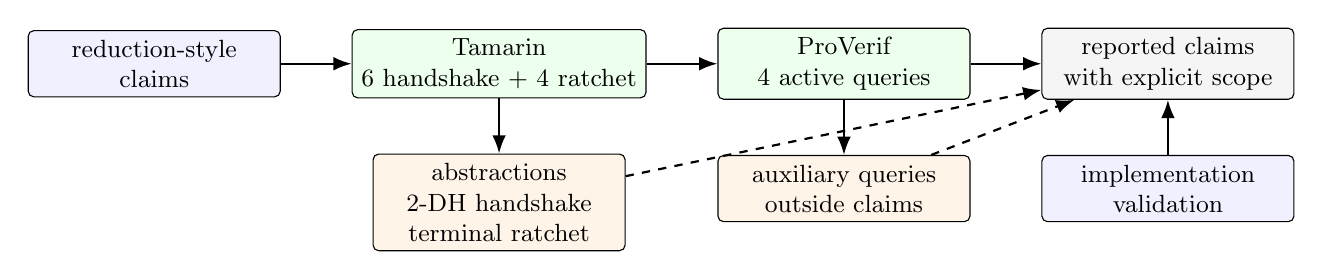
\begin{tikzpicture}[
  font=\small,
  source/.style={draw,rounded corners=2pt,align=center,minimum width=3.2cm,minimum height=0.78cm,fill=blue!6},
  model/.style={draw,rounded corners=2pt,align=center,minimum width=3.2cm,minimum height=0.78cm,fill=green!7},
  limit/.style={draw,rounded corners=2pt,align=center,minimum width=3.2cm,minimum height=0.78cm,fill=orange!9},
  claim/.style={draw,rounded corners=2pt,align=center,minimum width=3.2cm,minimum height=0.78cm,fill=gray!8},
  arrow/.style={-Latex,thick},
  node distance=0.7cm and 0.9cm
]
\node[source] (theory) {reduction-style\\claims};
\node[model,right=of theory] (tamarin) {Tamarin\\6 handshake + 4 ratchet};
\node[model,right=of tamarin] (proverif) {ProVerif\\4 active queries};
\node[claim,right=of proverif] (claims) {reported claims\\with explicit scope};

\node[limit,below=of tamarin] (abst) {abstractions\\2-DH handshake\\terminal ratchet};
\node[limit,below=of proverif] (stress) {auxiliary queries\\outside claims};
\node[source,below=of claims] (tests) {implementation\\validation};

\draw[arrow] (theory) -- (tamarin);
\draw[arrow] (tamarin) -- (proverif);
\draw[arrow] (proverif) -- (claims);
\draw[arrow] (tamarin) -- (abst);
\draw[arrow] (proverif) -- (stress);
\draw[arrow] (tests) -- (claims);
\draw[arrow,dashed] (abst) -- (claims);
\draw[arrow,dashed] (stress) -- (claims);
\end{tikzpicture}%
}
\caption{Formal-evidence map. The manuscript combines reduction-style
arguments, scoped symbolic models, and implementation validation. Abstractions
and auxiliary queries are shown separately from the claims counted as verified
evidence.}\label{fig:formal-evidence-map}
\end{figure}


% ═════════════════════════════════════════════════════════════
% 8. IMPLEMENTATION
% ═════════════════════════════════════════════════════════════
\section{Implementation}\label{sec:implementation}

The evaluated implementation follows the protocol decomposition used in the
preceding sections. Its role in this paper is not to serve as a proof object,
but to demonstrate that the mathematical state machine can be realized with
explicit parsing, rejection, erasure, replay, and persistence boundaries. The
implementation is organized around the following architectural responsibilities.

\begin{table}[H]
\centering
\caption{Implementation architecture.}\label{tab:modules}
\small
\begin{tabularx}{\textwidth}{@{}p{0.27\textwidth}Y@{}}
\toprule
Layer & Responsibility \\
\midrule
Core definitions & Versioning, protocol constants, error semantics, and bounded input sizes. \\
Cryptographic layer & Primitive instantiations for X25519, Ed25519, ML-KEM-768, HKDF, HMAC, AES-256-GCM-SIV, secure memory, and validation routines. \\
Identity and pre-key layer & Identity generation, signed pre-key handling, one-time pre-key selection, and responder bundle construction. \\
Session protocol layer & Hybrid pre-key agreement, root/chain ratchets, envelope processing, replay windows, and sealed-state import/export. \\
Validation boundary & Public-key validation, malformed-input rejection, downgrade handling, timestamp normalization, and state-transition atomicity checks. \\
External interface layer & A narrow interface for creating identities, initiating sessions, encrypting/decrypting messages, and serializing state. \\
\bottomrule
\end{tabularx}
\end{table}

\begin{figure}[H]
\centering
\resizebox{\textwidth}{!}{%
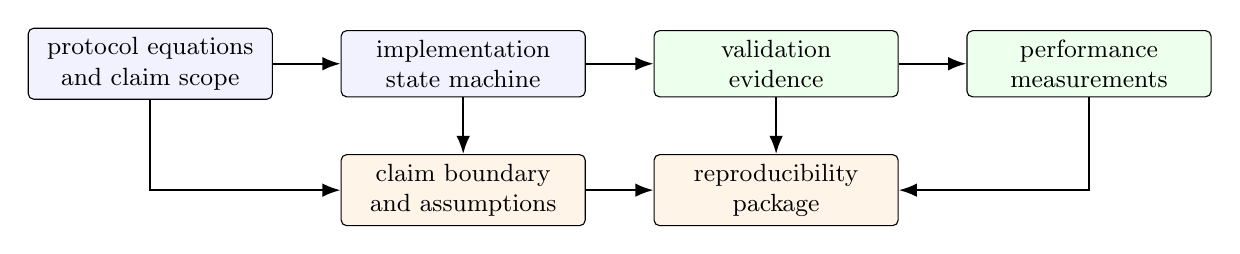
\begin{tikzpicture}[
  font=\small,
  box/.style={draw,rounded corners=2pt,align=center,minimum width=3.1cm,minimum height=0.78cm,fill=blue!5},
  evidence/.style={draw,rounded corners=2pt,align=center,minimum width=3.1cm,minimum height=0.78cm,fill=green!7},
  review/.style={draw,rounded corners=2pt,align=center,minimum width=3.1cm,minimum height=0.78cm,fill=orange!9},
  arrow/.style={-Latex,thick},
  node distance=0.72cm and 0.86cm
]
\node[box] (spec) {protocol equations\\and claim scope};
\node[box,right=of spec] (impl) {implementation\\state machine};
\node[evidence,right=of impl] (checks) {validation\\evidence};
\node[evidence,right=of checks] (perf) {performance\\measurements};

\node[review,below=of impl] (boundary) {claim boundary\\and assumptions};
\node[review,below=of checks] (repro) {reproducibility\\package};

\draw[arrow] (spec) -- (impl);
\draw[arrow] (impl) -- (checks);
\draw[arrow] (checks) -- (perf);
\draw[arrow] (spec) |- (boundary);
\draw[arrow] (impl) -- (boundary);
\draw[arrow] (checks) -- (repro);
\draw[arrow] (perf) |- (repro);
\draw[arrow] (boundary) -- (repro);
\end{tikzpicture}%
}
\caption{Implementation-evidence map. Executable validation and performance
measurements are used to support the stated implementation scope. They do
not replace the reduction-style claims or symbolic models.}\label{fig:implementation-evidence-map}
\end{figure}

\subsection{Cryptographic Library Choices}

\begin{table}[H]
\centering
\caption{Concrete primitive choices in the reference implementation.}\label{tab:deps}
\small
\begin{tabularx}{\textwidth}{@{}p{0.28\textwidth}Y@{}}
\toprule
Primitive & Implementation note \\
\midrule
X25519 and Ed25519 & Constant-time curve operations with public-key validation and protected handling of private material where supported. \\
ML-KEM-768 & FIPS~203 KEM used for initial and ratchet-level post-quantum contributions. Deterministic generation is restricted to reproducibility vectors. \\
AES-256-GCM-SIV & RFC~8452 misuse-resistant AEAD for payloads, metadata, and sealed state. \\
HKDF-SHA256 and HMAC-SHA256 & RFC~5869 and RFC~2104 constructions with explicit domain-separated labels. \\
Serialization & Length-bounded Protocol Buffers encoding with a fixed maximum message size. \\
Secret handling & Automatic and explicit zeroization of temporary key material, with platform memory protection for long-lived secrets where supported. \\
\bottomrule
\end{tabularx}
\end{table}

\subsection{Secure Memory Management}

Key material is protected at multiple levels:

\begin{enumerate}
  \item \textbf{Memory protection for long-lived secrets.} Long-lived DH and ML-KEM secret keys
  are stored through a memory-protection layer. Unix-like builds use a bounded,
  preallocated page-locked pool and request crash-dump exclusion where the
  platform provides it. Failure to establish or allocate from that pool is not
  silently downgraded to pageable memory. The iOS and Windows backends use
  heap storage with automatic zeroization because this Unix locking path is not
  selected on those targets.

  \item \textbf{Scope-bound zeroization.} Intermediate key material, including HKDF
  extract outputs and chain-key copies, is wrapped so that it is zeroized when it
  leaves scope, including error paths.

  \item \textbf{Immediate zeroization of consumed secrets.} DH shared secrets, hybrid input-keying
  buffers, classical shared secrets, and ML-KEM shared secrets are explicitly
  zeroized immediately after their consuming derivation.

  \item \textbf{Timestamp rounding.} Nanosecond fields in message timestamps are set to zero to reduce device fingerprinting through timing data.
\end{enumerate}

\subsection{ML-KEM-768 Integration}\label{sec:kyber-impl}

The ML-KEM-768 integration has three protocol-relevant points that affect the
validation boundary:

\begin{itemize}
  \item \textbf{Self-testing.} Random ML-KEM key generation is followed by an immediate encapsulate/decapsulate round-trip with constant-time shared secret comparison. Deterministic seeded generation is reserved for reproducible vectors. The self-test detects KEM correctness failures, including randomness-source, implementation, or integration faults that cause encapsulation and decapsulation to disagree.

  \item \textbf{Deterministic vectors.} Deterministic KEM generation is used
  only to produce reproducible vectors from an explicit seed. Normal protocol
  execution uses fresh randomness and does not rely on global deterministic
  hooks.

  \item \textbf{Bandwidth overhead.} Each hybrid ratchet step carries $1{,}184 + 1{,}088 + 32 = 2{,}304$ bytes of cryptographic material (ML-KEM public key + ciphertext + DH public key). Protocol Buffers field tags, length prefixes, the previous-chain-length value, and transport framing make the serialized increment slightly larger and value-dependent. For messaging applications with typical message sizes of 100--1{,}000 bytes, the raw cryptographic material alone represents an approximate 3--23$\times$ expansion per ratchet step.
\end{itemize}

% ═════════════════════════════════════════════════════════════
% 9. EVALUATION
% ═════════════════════════════════════════════════════════════
\section{Evaluation}\label{sec:evaluation}

\subsection{Performance Benchmarks}\label{sec:benchmarks}

Benchmarks are single-host Criterion measurements with 200 samples and
5-second measurement windows. They are hardware-dependent implementation-cost
snapshots, not security assumptions. The reproducibility material records the
platform, compiler and dependency context, raw measurement outputs, and the
inputs used for the summarized results in
\cref{tab:bench-core,tab:bench-payload,tab:bench-overhead}. A fixed
128-message, 256-byte traffic profile is also used to compare handshake-only
post-quantum key exchange, sparse chain-boundary rekeying, periodic
chain-boundary rekeying, and per-reply post-quantum rekeying under the same
measurement conditions.

The artifact manifest identifies the exact repository revision used for the
reported measurements and records the dirty-worktree summary, OS/kernel, CPU
summary, Rust compiler version, dependency lockfile hash, build-profile context,
and raw Criterion output in
\texttt{versions.txt}, \texttt{MANIFEST.txt}, and \texttt{SHA256SUMS}. The
tables below therefore summarize one auditable host profile rather than a
portable latency guarantee.

\begin{table}[H]
\centering
\caption{Core operation latencies.}\label{tab:bench-core}
\small
\begin{tabular}{@{}lr@{}}
\toprule
Operation & Latency \\
\midrule
Identity creation (5 OPKs) & $\sim$1.5\,ms \\
Full handshake (keygen + pre-key DH + ML-KEM + confirm) & $\sim$1.1\,ms \\
Handshake only (pre-created identity) & $\sim$0.7\,ms \\
Hybrid ratchet step (X25519 + ML-KEM-768) & $\sim$259\,$\mu$s \\
Encrypt 256\,B (same chain, no ratchet) & $\sim$17\,$\mu$s \\
Decrypt 256\,B (same chain, no ratchet) & $\sim$21\,$\mu$s \\
\midrule
ML-KEM-768 keygen & $\sim$80\,$\mu$s \\
ML-KEM-768 encapsulate & $\sim$100\,$\mu$s \\
ML-KEM-768 decapsulate & $\sim$90\,$\mu$s \\
X25519 scalar multiplication & $\sim$50\,$\mu$s \\
HKDF-SHA256 (32\,B output) & $\sim$2\,$\mu$s \\
\midrule
Session export (sealed) & $\sim$30\,$\mu$s \\
Session import (sealed) & $\sim$35\,$\mu$s \\
Shamir split (3-of-5, 32\,B) & $\sim$5\,$\mu$s \\
Shamir reconstruct (3-of-5, 32\,B) & $\sim$3\,$\mu$s \\
\bottomrule
\end{tabular}
\end{table}

\begin{table}[H]
\centering
\caption{Steady-state envelope decrypt latency by payload size.}\label{tab:bench-payload}
\small
\begin{tabular}{@{}rr@{}}
\toprule
Payload Size & Decrypt Latency \\
\midrule
64\,B & $\sim$35\,$\mu$s \\
256\,B & $\sim$38\,$\mu$s \\
1\,KiB & $\sim$45\,$\mu$s \\
4\,KiB & $\sim$60\,$\mu$s \\
16\,KiB & $\sim$120\,$\mu$s \\
64\,KiB & $\sim$350\,$\mu$s \\
256\,KiB & $\sim$1.2\,ms \\
1\,MiB & $\sim$4.5\,ms \\
\bottomrule
\end{tabular}
\end{table}

\begin{table}[H]
\centering
\caption{Ratchet overhead comparison.}\label{tab:bench-overhead}
\small
\begin{tabular}{@{}lr@{}}
\toprule
Component & Latency \\
\midrule
X25519 DH scalar multiplication (classical baseline) & $\sim$50\,$\mu$s \\
ML-KEM-768 encap + decap (PQ overhead) & $\sim$190\,$\mu$s \\
Full hybrid ratchet step (DH + ML-KEM + HKDF + encrypt) & $\sim$259\,$\mu$s \\
\midrule
Alternating throughput (ratchet every message, 256\,B) & $\sim$280\,$\mu$s/msg \\
Burst decrypt throughput (pre-generated envelopes, 256\,B) & $\sim$15\,$\mu$s/msg \\
\bottomrule
\end{tabular}
\end{table}

\paragraph{Analysis}
In these measurements, a hybrid ratchet step costs about $259\,\mu$s, versus about $50\,\mu$s for X25519 alone. Steady-state same-direction burst decrypts measure about $15\,\mu$s/msg. Alternating 256-byte messages, which time encryption and decryption in the loop, measure about $280\,\mu$s/msg. The full handshake measures about $1.1$\,ms on the benchmark host.

\subsection{Executable Validation}\label{sec:tests}

The pinned implementation snapshot contains 750 default test scenarios.
\Cref{tab:tests} reports the 556 non-VoIP scenarios used in the manuscript's
validation ledger. The excluded 194 VoIP scenarios exercise a separate media
state machine. The reported set also contains engineering checks outside the
formal two-party model. Only the checks mapped in \cref{tab:test-proof-mapping}
support claims about the two-party protocol.

\begin{table}[H]
\centering
\caption{Non-VoIP executable validation reported for the pinned snapshot.}\label{tab:tests}
\small
\begin{tabularx}{\textwidth}{@{}Xr@{}}
\toprule
Category & Scenarios \\
\midrule
Primitive and protocol checks & 36 \\
External-interface checks & 71 \\
End-to-end protocol-state scenarios & 392 \\
Adversarial and negative-session scenarios & 40 \\
Header, time, malformed-input, and property scenarios & 13 \\
Additional compatibility scenarios & 4 \\
\midrule
\textbf{Reported validation scenarios} & \textbf{556} \\
\bottomrule
\end{tabularx}
\end{table}

\paragraph{Property-based validation}
Six property-based checks generate random inputs across a range of parameters:
message counts (1--50), payload sizes (0--4{,}096~bytes), direction patterns,
Shamir SSS parameters, and message permutations. These complement the
deterministic checks by exploring the input space more broadly.

\paragraph{Security-property coverage mapping}
\Cref{tab:test-proof-mapping} maps each reduction-style security claim to executable
checks that exercise the corresponding concrete invariants:

\begin{table}[H]
\centering
\caption{Validation mapping: formal properties and implementation coverage.}\label{tab:test-proof-mapping}
\small
\begin{tabularx}{\textwidth}{@{}L{0.28\textwidth}Y@{}}
\toprule
Security Property & Implementation evidence \\
\midrule
Hybrid combiner (\cref{thm:hybrid-combiner}) & Initiator/responder agreement checks, deterministic-vector checks, and known-answer checks for hybrid derivation. \\
AKE security (\cref{thm:ake}) & Full handshake agreement, bilateral key confirmation, malformed-bundle rejection, and reflection-rejection checks. \\
Forward secrecy (\cref{thm:fs}) & Old-chain-key isolation and multi-step ratchet-recovery checks. \\
Post-compromise security (\cref{thm:pcs}) & Post-compromise ratchet recovery and delayed-delivery recovery checks across multiple ratchet steps. \\
Message security (\cref{thm:msg-security}) & Envelope AEAD checks, message round trips, malformed-envelope rejection, and property-based AEAD/message round trips. \\
Replay resistance (\cref{thm:replay}) & Duplicate-ciphertext rejection, persisted replay-window checks, and old-epoch rejection. \\
\bottomrule
\end{tabularx}
\end{table}


% ═════════════════════════════════════════════════════════════
% 10. OPERATIONAL INVARIANTS
% ═════════════════════════════════════════════════════════════
\section{Operational Conditions for the Implementation}\label{sec:operational-invariants}

The claims in \cref{sec:proofs} concern an abstract two-party session protocol.
The implementation checks in \cref{sec:implementation,sec:evaluation} examine
whether parsing, persistence, and error handling preserve the state assumptions
used by those claims. The required operational conditions are stated below.

\paragraph{Reject without state movement}
For syntactically invalid input, the required implementation semantics is
a pure rejection:
\begin{equation}\label{eq:reject-no-state}
  \mathsf{Handle}(S, C) = (\bot, S)
  \qquad\text{for every ciphertext or frame } C \notin \mathcal{L}_{\mathrm{AuraProtocol}} .
\end{equation}
Here $\mathcal{L}_{\mathrm{AuraProtocol}}$ is the set of well-formed protocol
frames with valid version tags, fixed-length X25519 and ML-KEM fields,
bounded counters, and a syntactically present ratchet header whenever the
message type requires one. The implementation checks those conditions
before any secret state is advanced. In particular, malformed protobuf
fields, unsupported versions, incorrect public-key lengths, oversized
payloads, missing ratchet material, and failed AEAD authentication must
not increment message counters, change replay windows, cache partial
keys, or rotate the root key. This invariant is what allows the formal
model to treat malformed traffic as absence of an accepted event rather
than as a third kind of state transition.

\paragraph{Atomic acceptance}
For valid traffic, acceptance is modeled as a single transition from
state $S_i$ to state $S_{i+1}$. The implementation has to preserve the
same abstraction even though it performs parsing, decryption, replay
checks, chain-key updates, metadata-key updates, and sealed-state export
as separate instructions. The required order is:
\begin{equation}\label{eq:accept-atomic}
  \mathsf{Verify}(C,S_i)=1
  \;\Longrightarrow\;
  \mathsf{Persist}(S_{i+1}) \prec \mathsf{Release}(M),
\end{equation}
unless the caller provides an equivalent durable transaction boundary.
If plaintext were released before replay state and chain state became
durable, a process crash could allow the same ciphertext to be accepted
again after restart. That would not contradict AEAD security or HKDF
pseudorandomness. It would violate the state premise of the replay
claim. This is why sealed state, the external monotonic counter, and
idempotent restore handling are part of the protocol evidence rather than
mere storage convenience.

\paragraph{Out-of-order delivery}
Asynchronous messaging cannot rely on FIFO transport. A delayed message
may arrive after a peer has already sent a new ratchet header, and an old
ciphertext may be replayed after a sealed-state import. The implementation
therefore binds skipped message keys and cached metadata keys to the
epoch in which they were derived. Accepting an old but still admissible
message must not roll the root key backward, reinterpret a metadata key
under a later epoch, or make a previously rejected ciphertext valid in a
new state. Bounded caches are part of the same invariant: they prevent an
attacker from forcing unbounded retention of old chain material and make
the replay window a concrete system parameter rather than an implicit
infinite buffer.

\paragraph{Key-directory and downgrade behavior}
The pre-key directory is not trusted to define the peer's identity. It can
delay updates, replay an old signed pre-key, omit a KEM public key, or
serve different bundles to different clients. Aura Protocol's claim is therefore
conditional on identity verification and on a policy decision that the
peer is expected to support the hybrid profile. Under that policy,
absence or substitution of KEM material is a visible protocol failure, not
a silent fallback to a weaker transcript. This distinction matters for
the harvest-now-decrypt-later claim: the hybrid argument applies to
sessions whose transcript actually contains the ML-KEM contribution
specified in \cref{sec:handshake}.

\paragraph{Why the tests are scoped}
The 556 validation scenarios in \cref{tab:tests} are reported only insofar as
they exercise the invariants above: domain separation, ratchet atomicity,
replay-window persistence, sealed-state freshness, malformed-input rejection,
and negative session behavior. Other engineering checks do not enlarge the
security claim. This keeps the empirical results aligned with the exact
two-party protocol analyzed in \cref{sec:security-model}. Broader product
surfaces require their own state models before analogous claims can be made.


% ═════════════════════════════════════════════════════════════
% 11. COMPARISON WITH CURRENT POST-QUANTUM MESSAGING BASELINES
% ═════════════════════════════════════════════════════════════
\section{Comparison with Current Post-Quantum Messaging Baselines}\label{sec:comparison}

For a 2026 comparison, PQXDH is no longer the sole baseline. It is a
handshake-level post-quantum upgrade, whereas Signal \SPQR{}/Triple Ratchet
and Apple \PQThree{} move post-quantum material into the ongoing evolution of
the session state. The table below separates where PQ entropy enters the
protocol, how PCS is recovered after compromise, and what public evidence
supports the design.

\begin{table}[H]
\centering
\caption{Positioning of Aura Protocol against current post-quantum messaging
baselines.}\label{tab:sota-comparison}
\scriptsize
\setlength{\tabcolsep}{2pt}
\begin{tabularx}{\textwidth}{@{}L{0.16\textwidth}L{0.19\textwidth}L{0.18\textwidth}L{0.17\textwidth}Y@{}}
\toprule
Protocol & Where PQ material is used & PCS after compromise & Public evidence & Implication for Aura Protocol \\
\midrule
Signal X3DH/Double Ratchet~\cite{signal-x3dh,signal-double-ratchet} &
Not used &
Classical PCS through the DH ratchet &
Open specifications and academic analyses &
Baseline FS/PCS model, but not quantum-resistant. \\
\addlinespace
Signal PQXDH~\cite{signal-pqxdh} &
Initial handshake &
No renewed PQ contribution after the handshake &
Open specification &
Handshake-only baseline for initial harvest-now-decrypt-later protection, not for PQ-PCS in a long-lived channel. \\
\addlinespace
Signal \SPQR{}/Triple Ratchet~\cite{signal-spqr,signal-double-ratchet,mlkem-braid,signal-spqr-artifact} &
Sparse PQ ratchet alongside the classical Double Ratchet &
PQ-PCS through SCKA epochs governed by ML-KEM Braid state and chunk/codeword delivery &
Open specifications, public SPQR reference material, and Signal engineering notes &
Open Signal-family baseline for ongoing PQ state evolution. \\
\addlinespace
Apple \PQThree{}~\cite{apple-pq3,stebila-pq3,linker-pq3} &
Initial establishment and periodic in-band rekeying &
Published analyses claim FS/PCS against classical and quantum adversaries &
Public design description, reduction-style analysis, and Tamarin analysis. Closed implementation &
Deployed industrial baseline for periodic in-band post-quantum rekeying. \\
\addlinespace
\textbf{Aura Protocol} &
Hybrid handshake and KEM rotation at directed ratchet boundaries &
Classical recovery after the next honest directed step. Hybrid recovery after a step using a post-compromise KEM key &
Six reduction-style claims, scoped Tamarin/ProVerif results, and executable validation &
Explicit KEM-key binding, per-epoch metadata encryption, and state-machine validation boundaries. \\
\bottomrule
\end{tabularx}
\end{table}

\begin{table}[H]
\centering
\caption{Compact comparison against nearest post-quantum messaging baselines.}
\label{tab:comparison}
\scriptsize
\begin{tabularx}{\textwidth}{@{}L{0.22\textwidth}YYYY@{}}
\toprule
Feature & PQXDH & \SPQR{} & \PQThree{} & \textbf{Aura Protocol} \\
\midrule
PQ contribution after handshake & No & Yes & Yes & \textbf{Yes} \\
PQ update schedule & One-time KEM & Sparse PQ ratchet & Periodic in-band rekeying & \textbf{KEM rotation at ratchet boundaries} \\
PQ-material binding & Initial KEM/session transcript & Braid authenticator MACs over header/ciphertext state & Authenticated in-band PQ rekeying in public analyses & \textbf{Ratchet KEM public key in HKDF info, AEAD-confirmed by the next message} \\
Separate envelope-metadata AEAD & Not specified by PQXDH & Not the focus of public Triple Ratchet/SPQR specs & PQ3 discusses padding and delivery receipts, not this envelope-key split & \textbf{Separate per-epoch metadata key} \\
Reference implementation & Specification & Public SPQR specifications and reference material & Public design, closed implementation & \textbf{Open reference implementation with validation material} \\
Formalized PQ-PCS delay & No & SCKA epoch analysis & Published PQ3 analysis & \textbf{PCS boundary for local vs.\ two-endpoint compromise} \\
\bottomrule
\end{tabularx}
\end{table}

The comparison identifies Aura Protocol's specific design role. Signal \SPQR{} provides
the closest Signal-family baseline for sparse post-quantum state evolution,
whereas Apple \PQThree{} represents a deployed industrial design with periodic
in-band rekeying. Aura Protocol uses a directed-ratchet construction in which
fresh KEM material enters the channel state at ratchet
boundaries, the advertised KEM public key is bound into the transcript without
an extra signature, and metadata has its own rotating key. The implementation
and formal models make this construction independently inspectable.

\subsection{Ratcheting Strategy}

The relevant design choice is trigger granularity. Classical DH ratchets advance
when a new peer DH public key is received~\cite{signal-double-ratchet}, while
sparse post-quantum schedules amortize KEM work across longer state epochs.
Aura Protocol uses per-direction hybrid ratcheting. After every received
message, the next send triggers a full X25519 and ML-KEM transition. Each
direction change therefore installs a new root key and limits a chain-key
compromise to the affected direction and epoch. The KEM contribution is also
renewed beyond the initial handshake. Following local compromise, classical
PCS begins at the next honest transition. Following two-endpoint compromise,
hybrid recovery waits until a directed transition uses peer DH and KEM material
generated after the compromise.

\paragraph{Cost}
Each hybrid ratchet step adds $\sim$259\,$\mu$s of computation and 2{,}304 bytes of raw cryptographic material (1{,}184 bytes for the ML-KEM public key, 1{,}088 bytes for the ML-KEM ciphertext, and 32 bytes for the DH public key), plus serialization framing. For interactive messaging with alternating messages, the measured profile is $\sim$280\,$\mu$s/msg. The $\sim$15\,$\mu$s/msg burst number is a decrypt-only measurement over pre-generated same-direction envelopes.

\subsection{PCS Recovery: 1-Step vs.\ 2-Step}

Classical DH ratchets achieve PCS once an uncompromised DH contribution
enters the root chain. Aura Protocol separates two cases. If only the local endpoint
state is compromised, the next honest directed step gives 1-step
\emph{classical} PCS via $\GapCDH$ on fresh DH material. If both endpoints'
epoch state is compromised, the first directed step may still use peer
ratchet state exposed before recovery. Hybrid recovery is claimed only once a
directed step uses peer DH and KEM material generated after the compromise.
\Cref{thm:pcs} formalizes these recovery conditions.

\subsection{Identity Binding}

Authenticated pre-key messaging protocols bind long-term identities through
signed pre-key material, authenticated key-agreement transcripts, and associated
data. Aura Protocol makes this binding explicit by deriving an identity-binding
hash
\[
  \mathit{ibh} =
    \SHA(\domain{Aura-Identity-Binding}\concat \mathrm{sort}(\cdot))
\]
and embedding it in every AEAD additional-data field. Including both identities
prevents cross-session identity confusion. Lexicographic sorting gives a stable
unordered peer-set value, while transcript and key-confirmation domains retain
the initiator and responder roles. The dedicated domain label prevents
cross-protocol reuse, and including the hash in both metadata and payload AAD
applies the same binding to both encrypted layers.


% ═════════════════════════════════════════════════════════════
% 11. DISCUSSION
% ═════════════════════════════════════════════════════════════
\section{Discussion}\label{sec:discussion}

\subsection{Bandwidth Overhead}

The primary cost of per-ratchet hybrid key exchange is bandwidth. Each ratchet
step carries 2{,}304 bytes of raw DH/KEM material before serialization framing,
which is approximately a $23\times$ increase
for a message carrying approximately 100 bytes of application data. Bursts
amortize this cost because only the first message in a direction carries the
ratchet header. Later messages in the same epoch have no KEM header. The
protocol assumes no compression of KEM fields because compression would require
separate security and side-channel analysis. Replacing ML-KEM-768 with
ML-KEM-512 would reduce the comparable header to 1{,}600 bytes
($800 + 768 + 32$), but would also lower the post-quantum target to NIST Level~1.

\subsection{2-Step Hybrid PCS}

The 2-step hybrid PCS recovery follows from the directed KEM-public-key ratchet used in Aura Protocol. After a local compromise, the first honest directed step can restore classical security through a fresh DH contribution. After full two-endpoint state compromise, however, the peer DH and KEM state used by that first directed step may already be exposed, so no one-step recovery is claimed. Full hybrid recovery is restored on a later directed step that uses peer DH and KEM material generated after the compromise.

Within this KEM-public-key ratchet pattern, one-step hybrid recovery would
require a different schedule, such as simultaneous KEM-key transport, an
acknowledged key update, or another post-quantum SCKA design. The analysis does
not claim that the two-step delay is a lower bound for other ratchet designs.

\subsection{ProVerif Stress Checks}

The ProVerif model discharges the primary proof-scope queries reported in
\cref{tab:proverif}, but the stress checks remain outside that count. Injective
authentication exceeds the practical scope of the four-DH ProVerif model within
the artifact budget. Broad unpartnered message integrity is false for the active
trace in which an adversary establishes its own session and delivers its own
plaintext. Raw KEM shared-secret secrecy after the corresponding KEM secret key
is revealed is false by decapsulation semantics, and therefore is not the
forward-secrecy property claimed here. The claimed properties are carried by the
Tamarin authentication, secrecy, and PCS abstractions, the reduction-style arguments, and
the executable validation categories described above.

\subsection{Kyber/ML-KEM Terminology}

The protocol is described in terms of ML-KEM-768. Earlier Kyber terminology may
appear in legacy implementation identifiers, but no Kyber-specific security
claim is made here. The reference implementation is not a certified FIPS
module. A certified-provider migration is intended to be confined to the KEM
wrapper and validation boundary while preserving protocol messages and proof
assumptions. The hybrid combiner's security relies on $\INDCCA$ security of the
KEM, which ML-KEM provides.

\subsection{Operational Profiles}

The intended operating point is asynchronous text messaging. In that setting,
a full hybrid ratchet on direction change keeps the recovery rule simple while
amortizing the 2.3~KB of raw ratchet material over bursts of messages sent in the same
direction. After a local state compromise, the first honest ratchet step restores
the classical DH contribution. After full two-endpoint state compromise, recovery
is tied to a later directed step that uses post-compromise peer DH and KEM
material.

Latency-constrained profiles with a hard per-packet budget are a separate design
point. The handshake can still establish an authenticated hybrid secret, but the
ratchet schedule would need its own timing, acknowledgement, and loss model. The
two-party messaging claims should not be read as proofs for such a profile
unless that profile carries its own state machine and recovery argument.

Long-lived desktop and server-side sessions put pressure on a different part of
the design: sealed state. A valid encrypted state blob is not necessarily a
fresh state blob. Backup restore, VM snapshots, and storage migration can replay
an old but correctly authenticated state. The sealed-state counter is therefore
part of the protocol integration rather than a serialization detail. Without an
external monotonic value, AEAD and HMAC authenticate the blob but cannot tell a
current state from an older valid one.

Multi-device accounts introduce another boundary. The current model treats a
session as a two-party channel between two devices. If one user has several
devices, the system has to decide whether to run separate pairwise sessions,
fan out messages through a Sesame-like session manager, or introduce a separate
multi-device state-management layer. These choices affect replay windows, identity binding,
device removal, and sealed-state freshness. They are deployment-level choices, and
they should not be folded into the two-party claims.

\subsection{Reproducibility and Traceability}

The computational arguments, symbolic models, and executable checks answer
different questions. The arguments state the primitive assumptions and
security losses. Tamarin and ProVerif examine selected trace properties under
documented abstractions. The executable scenarios cover serialization, nonce
discipline, replay state, skipped-key handling, and rejection of malformed
envelopes. Table~\ref{tab:test-proof-mapping} links these checks to the protocol
properties they exercise without treating test success as a cryptographic
reduction.

This traceability also defines the work required after a protocol change. A
change to a key derivation must be reflected in the argument and symbolic
models. A change to framing or persistence requires new executable checks. The
same discipline makes comparison with Signal \SPQR{} and Apple \PQThree{}
concrete: Aura Protocol exposes ratchet state, KEM-key binding, metadata-key
rotation, and sealed-state rollback handling in one reproducible package.

The accompanying reproducibility material is organized to rebuild the paper,
rerun the validation suite, rerun the symbolic models, and reproduce the
benchmark summaries. Deterministic vectors cover HKDF, AES-GCM-SIV, seeded
ML-KEM public-key generation, master-key identity derivation, the full
handshake transcript, the first post-handshake envelope, the first
DH+KEM-ratchet envelope, and multi-epoch delayed-delivery envelopes. The
archived material records tool versions, manifests, checksums, formal-model
logs, paper-build logs, and benchmark summaries. These artifacts are structured
so that independent reviewers can compare model assumptions with the
implementation paths exercised by the validation suite.

\subsection{Limitations}

\begin{table}[tbp]
\centering
\caption{Ranked limitations and deployment effect.}
\label{tab:limitations}
\footnotesize
\begin{tabularx}{\textwidth}{@{}L{0.16\textwidth}L{0.24\textwidth}Y@{}}
\toprule
Severity & Limitation & Deployment effect and treatment \\
\midrule
High & Classical identity authentication. & Ed25519 identity and SPK signatures leave active impersonation outside the post-quantum claim once a CRQC can forge signatures. A migration to ML-DSA or another post-quantum signature scheme is required for post-quantum authentication. The ratchet analysis remains a confidentiality argument under the current classical-authentication assumptions. \\
High & Sealed-state freshness. & AEAD and state HMACs authenticate serialized state but cannot distinguish a current blob from an older valid blob. Rollback protection therefore requires an external monotonic counter or equivalent freshness anchor. \\
Medium & Key-directory and TOFU assumptions. & The protocol assumes identity verification and policy enforcement for the hybrid profile. Directory equivocation, stale bundles, and downgrade attempts are treated as deployment risks unless the client detects and rejects them. \\
Medium & Single-device two-party scope. & The analyzed model is one device talking to one device. Multi-device fan-out, Sesame-like session management, and group messaging require separate state machines and proofs. \\
Medium & Ratchet cost and bandwidth. & Per-direction KEM rotation carries 2.3~KB of raw cryptographic material plus serialization framing and adds about $259\,\mu$s of ratchet work on the measured host. Lower-frequency ratchet schedules may be attractive but need their own PCS and cost statements. \\
Medium & Symbolic-model abstraction. & Tamarin and ProVerif support scoped claims, not complete protocol verification. The executable validation suite checks concrete parsing and rollback behavior, but it does not replace reductions or platform audits. \\
\bottomrule
\end{tabularx}
\end{table}


% ═════════════════════════════════════════════════════════════
% 12. CONCLUSION
% ═════════════════════════════════════════════════════════════
\section{Conclusion}\label{sec:conclusion}

Aura Protocol shows that post-quantum confidentiality can be incorporated into
the continuing state evolution of a two-party secure-messaging protocol without
treating the KEM as a one-time handshake add-on. The construction refreshes
ML-KEM material at directed ratchet boundaries, binds each advertised KEM public
key into the HKDF transcript, separates payload and envelope-metadata keys, and
uses nonce-misuse-resistant AEAD for both message layers. The analysis identifies
different recovery points for local and two-endpoint compromise. Local recovery
obtains a fresh classical contribution at the next honest transition. Hybrid
recovery requires a later transition that uses peer DH and KEM material created
after the compromise.

Six reduction-style arguments state the computational assumptions behind the
construction. Ten Tamarin lemmas, three primary ProVerif queries, and one scoped
correspondence query examine reduced handshake, ratchet, secrecy, and
correspondence properties. Executable
validation covers parsing, persistence, replay handling, negative-state
behavior, and sealed-state import. Together these results connect the abstract
state transitions to the implemented two-party message path while preserving
the stated limits of each analysis.

The evaluated implementation indicates that the design is practical for
asynchronous messaging profiles. On the reported host, the full handshake takes
approximately $1.1$\,ms, alternating 256-byte messages cost about
$280\,\mu$s/msg, and steady-state same-direction decrypts cost about
$15\,\mu$s/msg. The 2{,}304 bytes of raw ratchet key and ciphertext material are the dominant deployment
cost for short messages. Post-quantum identity authentication, stronger
state-freshness anchors, multi-device operation, group messaging, mobile-class
measurements, and lower-frequency ratchet schedules remain outside the analyzed
construction. Aura Protocol therefore establishes an implementation-backed
design for continuing post-quantum confidentiality in a two-party stateful
channel, with its recovery delay and operational cost stated quantitatively.

\section*{Data and Software Availability}

The source code, validation material, formal models, reproducibility scripts,
benchmark definitions, and manuscript sources are available at
\url{https://github.com/oleksandrmelnychenko/aura-protected-protocol-rs}.
The evaluated implementation snapshot is
\href{https://github.com/oleksandrmelnychenko/aura-protected-protocol-rs/tree/b788e075b6f3558ce1c3bbdb66d724bb65960f8c}{commit \texttt{b788e07}}.
The reproduction script records tool versions and produces
\texttt{MANIFEST.txt}, \texttt{SHA256SUMS}, formal-model logs, benchmark
summaries, and deterministic vector outputs. Later repository revisions are not
part of the evaluated snapshot.

\section*{Funding}

The author declares that this research received no external funding.

\section*{CRediT Author Statement}

Oleksandr Melnychenko: conceptualization, methodology, software,
validation, formal analysis, investigation, writing--original draft,
writing--review and editing, and visualization.

\section*{Declaration of Competing Interest}

The author declares that there are no known competing financial
interests or personal relationships that could have appeared to
influence the work reported in this paper.

\section*{Declaration of Generative AI and AI-assisted technologies in the writing process}

OpenAI Codex was used during manuscript preparation to assist with
English-language editing, consistency checks, and minor \LaTeX{}
typesetting support. OpenAI Codex was not used as an authoritative
source for technical claims, references, equations, implementation
results, or experimental measurements. All protocol descriptions,
equations, references, tables, implementation details, and experimental
results were independently reviewed, verified, and approved by the
author, who takes full responsibility for the content of the article.


% ═════════════════════════════════════════════════════════════
% REFERENCES
% ═════════════════════════════════════════════════════════════
\bibliographystyle{elsarticle-num}
\begin{thebibliography}{99}

\bibitem{signal-x3dh}
M.~Marlinspike and T.~Perrin.
\newblock The {X3DH} key agreement protocol, revision~1.
\newblock Signal Technical Documentation, 2016.
\newblock \url{https://signal.org/docs/specifications/x3dh/}

\bibitem{cohn-gordon2020}
K.~Cohn-Gordon, C.~Cremers, B.~Dowling, L.~Garratt, and D.~Stebila.
\newblock A formal security analysis of the Signal messaging protocol.
\newblock \emph{Journal of Cryptology}, 33(4):1914--1983, 2020.
\newblock \url{https://doi.org/10.1007/s00145-020-09360-1}

\bibitem{svystun2025dytam}
S.~Svystun, L.~Scis{\l}o, M.~Pawlik, O.~Melnychenko, P.~Radiuk, O.~Savenko, and A.~Sachenko.
\newblock DyTAM: Accelerating wind turbine inspections with dynamic UAV trajectory adaptation.
\newblock \emph{Energies}, 18(7):1823, 2025.
\newblock \url{https://doi.org/10.3390/en18071823}

\bibitem{svystun2024thermal}
S.~Svystun, O.~Melnychenko, P.~Radiuk, O.~Savenko, A.~Sachenko, and A.~Lysyi.
\newblock Thermal and RGB images work better together in wind turbine damage detection.
\newblock \emph{International Journal of Computing}, 23(4):526--535, 2024.
\newblock \url{https://doi.org/10.47839/ijc.23.4.3752}

\bibitem{lysyi2025fire}
A.~Lysyi, A.~Sachenko, P.~Radiuk, M.~Lysyi, O.~Melnychenko, O.~Ishchuk, and O.~Savenko.
\newblock Enhanced fire hazard detection in solar power plants: an integrated UAV, AI, and SCADA-based approach.
\newblock \emph{Radioelectronic and Computer Systems}, (2):99--117, 2025.
\newblock \url{https://doi.org/10.32620/reks.2025.2.06}

\bibitem{fips203}
National Institute of Standards and Technology.
\newblock Module-lattice-based key-encapsulation mechanism standard ({ML-KEM}).
\newblock FIPS 203, 2024.
\newblock \url{https://csrc.nist.gov/pubs/fips/203/final}

\bibitem{shor1997}
P.~W.~Shor.
\newblock Polynomial-time algorithms for prime factorization and discrete logarithms on a quantum computer.
\newblock \emph{SIAM Journal on Computing}, 26(5):1484--1509, 1997.
\newblock \url{https://arxiv.org/abs/quant-ph/9508027}

\bibitem{signal-pqxdh}
E.~Kret and R.~Schmidt.
\newblock The {PQXDH} key agreement protocol, revision~3.
\newblock Signal Technical Documentation, 2024.
\newblock \url{https://signal.org/docs/specifications/pqxdh/}

\bibitem{signal-spqr}
G.~Connell and R.~Schmidt.
\newblock Signal Protocol and post-quantum ratchets.
\newblock Signal Blog, 2025.
\newblock \url{https://signal.org/blog/spqr/}

\bibitem{signal-double-ratchet}
T.~Perrin, M.~Marlinspike, and R.~Schmidt.
\newblock The Double Ratchet Algorithm, revision~4.
\newblock Signal Technical Documentation, 2025.
\newblock \url{https://signal.org/docs/specifications/doubleratchet/}

\bibitem{mlkem-braid}
R.~Schmidt.
\newblock The ML-KEM Braid Protocol.
\newblock Signal Technical Documentation, 2025.
\newblock \url{https://signal.org/docs/specifications/mlkembraid/}

\bibitem{apple-pq3}
Apple Security Engineering and Architecture.
\newblock iMessage with {PQ3}: The new state of the art in quantum-secure
messaging at scale.
\newblock Apple Security Research, 2024.
\newblock \url{https://security.apple.com/blog/imessage-pq3/}

\bibitem{stebila-pq3}
D.~Stebila.
\newblock Security analysis of the iMessage {PQ3} protocol.
\newblock Technical report, 2024.
\newblock \url{https://www.douglas.stebila.ca/research/papers/Apple-Stebila24/}

\bibitem{linker-pq3}
F.~Linker, R.~Sasse, and D.~Basin.
\newblock A Formal Analysis of Apple's iMessage {PQ3} Protocol.
\newblock In \emph{USENIX Security 2025}, pages 5015--5034.
\newblock \url{https://www.usenix.org/conference/usenixsecurity25/presentation/linker}

\bibitem{alwen2020}
J.~Alwen, S.~Coretti, and Y.~Dodis.
\newblock The double ratchet: Security notions, proofs, and modularization for the Signal protocol.
\newblock In \emph{EUROCRYPT 2019}, pages 129--158. Springer, 2019.
\newblock \url{https://doi.org/10.1007/978-3-030-17653-2_5}

\bibitem{bienstock2020}
A.~Bienstock, J.~Fairoze, S.~Garg, P.~Mukherjee, and S.~Raghuraman.
\newblock A more complete analysis of the Signal Double Ratchet algorithm.
\newblock In \emph{CRYPTO 2022}, pages 784--813. Springer, 2022.
\newblock \url{https://doi.org/10.1007/978-3-031-15802-5_27}

\bibitem{brendel2020}
J.~Brendel, M.~Fischlin, F.~G{\"u}nther, C.~Janson, and D.~Stebila.
\newblock Towards post-quantum security for Signal's {X3DH} handshake.
\newblock In \emph{Selected Areas in Cryptography -- SAC 2020}, pages 404--430. Springer, 2021.
\newblock \url{https://doi.org/10.1007/978-3-030-81652-0_16}

\bibitem{hashimoto2021}
K.~Hashimoto, S.~Katsumata, K.~Kwiatkowski, and T.~Prest.
\newblock An efficient and generic construction for Signal's handshake (X3DH): Post-quantum, state leakage secure, and deniable.
\newblock In \emph{PKC 2021}, pages 410--440. Springer, 2021.
\newblock \url{https://doi.org/10.1007/978-3-030-75248-4_15}

\bibitem{cecpq2}
A.~Langley.
\newblock CECPQ2.
\newblock Google Chrome experiment, 2018.
\newblock \url{https://www.imperialviolet.org/2018/12/12/cecpq2.html}

\bibitem{stebila2020}
D.~Stebila and M.~Mosca.
\newblock Post-quantum key exchange for the Internet and the Open Quantum Safe project.
\newblock In \emph{Selected Areas in Cryptography -- SAC 2016}, pages 14--37. Springer, 2017.
\newblock \url{https://doi.org/10.1007/978-3-319-69453-5_2}

\bibitem{bindel2019}
N.~Bindel, J.~Brendel, M.~Fischlin, B.~Goncalves, and D.~Stebila.
\newblock Hybrid key encapsulation mechanisms and authenticated key exchange.
\newblock In \emph{Post-Quantum Cryptography -- PQCrypto 2019}, pages 206--226. Springer, 2019.
\newblock \url{https://doi.org/10.1007/978-3-030-25510-7_12}

\bibitem{dowling2020}
B.~Dowling, M.~Fischlin, F.~G{\"u}nther, and D.~Stebila.
\newblock A cryptographic analysis of the {TLS} 1.3 handshake protocol.
\newblock \emph{Journal of Cryptology}, 34(4):37, 2021.
\newblock \url{https://doi.org/10.1007/s00145-021-09384-1}

\bibitem{meier2013}
S.~Meier, B.~Schmidt, C.~Cremers, and D.~Basin.
\newblock The {TAMARIN} prover for the symbolic analysis of security protocols.
\newblock In \emph{CAV 2013}, pages 696--701. Springer, 2013.
\newblock \url{https://doi.org/10.1007/978-3-642-39799-8_48}

\bibitem{blanchet2016}
B.~Blanchet.
\newblock Modeling and verifying security protocols with the applied pi calculus and {ProVerif}.
\newblock \emph{Foundations and Trends in Privacy and Security}, 1(1--2):1--135, 2016.
\newblock \url{https://bblanche.gitlabpages.inria.fr/publications/BlanchetFnTPS16.html}

\bibitem{sealed-sender}
J.~Lund.
\newblock Technology preview: Sealed Sender for Signal.
\newblock Signal Blog, 2018.
\newblock \url{https://signal.org/blog/sealed-sender/}

\bibitem{sphinx}
G.~Danezis and I.~Goldberg.
\newblock Sphinx: A compact and provably secure mix format.
\newblock In \emph{IEEE Symposium on Security and Privacy}, pages 269--282, 2009.
\newblock \url{https://doi.org/10.1109/SP.2009.15}

\bibitem{loopix}
A.~M.~Piotrowska, J.~Hayes, T.~Elahi, S.~Meiser, and G.~Danezis.
\newblock The Loopix anonymity system.
\newblock In \emph{USENIX Security 2017}, pages 1199--1216.
\newblock \url{https://www.usenix.org/conference/usenixsecurity17/technical-sessions/presentation/piotrowska}

\bibitem{rfc8452}
S.~Gueron, A.~Langley, and Y.~Lindell.
\newblock {AES-GCM-SIV}: Nonce misuse-resistant authenticated encryption.
\newblock RFC 8452, IETF, 2019.
\newblock \url{https://www.rfc-editor.org/rfc/rfc8452}

\bibitem{rogaway2006}
P.~Rogaway and T.~Shrimpton.
\newblock A provable-security treatment of the key-wrap problem.
\newblock In \emph{EUROCRYPT 2006}, pages 373--390. Springer, 2006.
\newblock \url{https://doi.org/10.1007/11761679_23}

\bibitem{rfc7748}
A.~Langley, M.~Hamburg, and S.~Turner.
\newblock Elliptic curves for security.
\newblock RFC 7748, IETF, 2016.
\newblock \url{https://www.rfc-editor.org/rfc/rfc7748}

\bibitem{krawczyk2010}
H.~Krawczyk.
\newblock Cryptographic extraction and key derivation: The {HKDF} scheme.
\newblock In \emph{CRYPTO 2010}, pages 631--648. Springer, 2010.
\newblock \url{https://doi.org/10.1007/978-3-642-14623-7_34}

\bibitem{rfc5869}
H.~Krawczyk and P.~Eronen.
\newblock {HMAC}-based extract-and-expand key derivation function ({HKDF}).
\newblock RFC 5869, IETF, 2010.
\newblock \url{https://www.rfc-editor.org/rfc/rfc5869}

\bibitem{lamacchia2007}
B.~LaMacchia, K.~Lauter, and A.~Mityagin.
\newblock Stronger security of authenticated key exchange.
\newblock In \emph{ProvSec 2007}, pages 1--16. Springer, 2007.
\newblock \url{https://doi.org/10.1007/978-3-540-75670-5_1}

\bibitem{canetti2001}
R.~Canetti and H.~Krawczyk.
\newblock Analysis of key-exchange protocols and their use for building secure channels.
\newblock In \emph{EUROCRYPT 2001}, pages 453--474. Springer, 2001.
\newblock \url{https://doi.org/10.1007/3-540-44987-6_28}

\bibitem{fips198}
National Institute of Standards and Technology.
\newblock The keyed-hash message authentication code ({HMAC}).
\newblock FIPS 198-1, 2008.
\newblock \url{https://doi.org/10.6028/NIST.FIPS.198-1}

\bibitem{rfc8032}
S.~Josefsson and I.~Liusvaara.
\newblock Edwards-curve digital signature algorithm ({EdDSA}).
\newblock RFC 8032, IETF, 2017.
\newblock \url{https://www.rfc-editor.org/rfc/rfc8032}

\bibitem{signal-spqr-artifact}
Signal Messenger.
\newblock SparsePostQuantumRatchet.
\newblock Public reference material, 2025.
\newblock \url{https://github.com/signalapp/SparsePostQuantumRatchet}

\end{thebibliography}

\end{document}
